% Springer Nature manuscript draft configured for Discover Artificial Intelligence.
\documentclass[pdflatex,sn-mathphys-num]{sn-jnl}

\usepackage{graphicx}
\usepackage{multirow}
\usepackage{amsmath,amssymb,amsfonts}
\usepackage{amsthm}
\usepackage{mathrsfs}
\usepackage[title]{appendix}
\usepackage{xcolor}
\usepackage{textcomp}
\usepackage{manyfoot}
\usepackage{booktabs}
\usepackage{algorithm}
\usepackage{algorithmicx}
\usepackage{algpseudocode}
\usepackage{listings}
\usepackage{tabularx}
\usepackage{array}
\usepackage{url}
\usepackage{placeins}

% --- FIX 1: theorem environments (were never declared in the original) ---
\theoremstyle{thmstyleone}
\newtheorem{proposition}{Proposition}
\theoremstyle{thmstylethree}
\newtheorem{definition}{Definition}

% Centered tabularx column (C = centered X)
\newcolumntype{C}{>{\centering\arraybackslash}X}

% --- FIX 3: restore standard LaTeX table environment, guarded so it cannot fail ---
\makeatletter
\@ifundefined{tableorg}{}{\let\table\tableorg \let\endtable\endtableorg}
\makeatother

% Relax float fractions so small tables never deadlock the float queue
\renewcommand\floatpagefraction{.3}
\renewcommand\topfraction{.95}
\renewcommand\bottomfraction{.95}
\renewcommand\textfraction{.05}

\raggedbottom

% Review copy: Discover Artificial Intelligence requests a minimum 12 pt font.
\makeatletter
\renewcommand\normalsize{\@setfontsize\normalsize{12pt}{14pt}}
\makeatother
\normalsize

\begin{document}

\title[Quality-Guarded Multi-Attribute Foundation Model Recommendation]{Quality-Guarded Multi-Attribute Foundation Model Recommendation: A Scoring Pipeline with Pareto Stratification}

\author*[1]{\fnm{Surbhi} \sur{Agrawal}}\email{surbhiagrwal.rvitm@rvei.edu.in}
\author[1]{\fnm{Divy} \sur{Chouksey}}\email{divychouksey136@gmail.com}

\affil*[1]{\orgdiv{Department of CSE (AI \& ML)}, \orgname{RV Institute of Technology \& Management}, \orgaddress{\city{Bangalore}, \country{India}}}

\abstract{Selecting a foundation model requires balancing quality, cost, latency, context, privacy, and availability, yet public leaderboards rank on a single dimension and linear weighted sums let cheap or fast models offset inadequate quality. We present a recommendation pipeline combining hard feasibility constraints, Pareto stratification, constant-elasticity-of-substitution (CES) aggregation, soft-knee percentile normalization, and a continuous quality-deficit penalty in place of threshold cliffs. We prove monotonicity and, under stated factor bounds, a quality-conditional score ceiling and properties of a bounded display mapping; we also show that Pareto dominance over the efficiency triplet implies score order only under a stated condition, with a counterexample outside it. On a frozen 47-model Agent Arena cohort, regret is measured against the leaderboard's net-improvement outcome, which does not price cost or latency. Under capability-first intent, the pipeline has the lowest point-estimate mean regret among the original unpenalized integrative baselines (0.09 versus 0.49), although paired intervals include zero. Corrected ablation leaves regret unchanged when the deficit factor is removed, but it rises to 1.28 when the frontier reward is removed (paired difference interval 0 to 2.49). Adding the same deficit factor and frontier reward to WSM also yields 0.09; adding the deficit factor alone to WSM or TOPSIS leaves regret at 0.49. Replacing CES with a linear aggregator leaves mean regret unchanged and also retains top-three overlap of 2/3. Under budget and balanced intents the pipeline trails several baselines; these are limitations because the outcome cannot adjudicate cost-sensitive preferences. A secondary common-utility analysis applies shared cost caps and an explicit utility to all methods, using weights that have not been validated against user choices. The results show outcome alignment on one cohort, not user-intent satisfaction.}

\keywords{Foundation models, quality-deficit penalty, Constant elasticity of substitution, Multi-attribute utility theory, Pareto optimality, recommendation systems, Model selection}

\maketitle

\section{Introduction}\label{sec:introduction}

The operational landscape of generative artificial intelligence is characterized by an expanding frontier of foundation models with divergent architectural specializations, parameter scales, deployment modalities, and cost structures \cite{bommasani2021opportunities, kaplan2020scaling}. Enterprise architects and system developers face a high-dimensional multi-criteria decision dilemma: selecting an optimal model is no longer a matter of querying the top of a general-purpose leaderboard. A production workflow may mandate sub-second response times for real-time customer interaction, multi-hundred-kilotoken context windows for complex codebases, air-gapped on-premises privacy, or aggressive unit economics for high-throughput batch extraction \cite{zheng2024judging}.

Despite the multidimensional nature of foundation model selection, existing evaluation tools and routing frameworks suffer from four critical structural deficiencies:
\begin{enumerate}
  \item \textbf{Single-Metric Myopia:} Public leaderboards typically rank models along a single aggregate dimension, such as Chatbot Arena Elo or standardized benchmark suites (e.g., MMLU, HumanEval, SWE-bench) \cite{hendrycks2020measuring, chen2021evaluating, jimenez2023swe}. These aggregate rankings ignore operational dimensions such as throughput (tokens per second), latency to first token, dollar cost per million tokens, context limits, and licensing compliance.
  \item \textbf{Compensatory Collapse in Linear Additive Utility:} When multi-criteria ranking is attempted, existing tools almost universally employ naive weighted linear arithmetic sums: $U = \sum w_i x_i$. Under linear aggregation, attributes are treated as perfect substitutes. A model with unacceptable task proficiency can outscore an elite frontier model simply because its low cost or rapid generation inflates its composite score. In mission-critical workflows, task quality is non-compensatory: exceptional affordability cannot compensate for defective reasoning.
  \item \textbf{Cliff Effects in Discontinuous Filtering:} While hard constraint filtering is essential, applying crude step penalties (e.g., penalizing a score by a flat 40\% if quality drops below an arbitrary threshold) creates severe instability. Models hovering marginally above or below the cutoff experience discontinuous ranking inversions.
  \item \textbf{Cohort Normalization Collapse and Tie Clumping:} Standard min-max normalization maps the empirical maximum to $1.0$, leaving scores acutely vulnerable to outlier distortion. Conversely, clipping values at a fixed upper percentile $P_{95}$ collapses all top-tier models onto identical $1.0$ normalized scores, destroying discriminatory power among elite alternatives. Similarly, hard display caps (e.g., $\min(99, S)$) generate artificial plateaus among top-scoring candidates.
\end{enumerate}

To overcome these structural limitations, this paper develops a principled, multi-attribute decision-analytic scoring methodology for foundation model recommendation. We draw theoretical inspiration from the \emph{Cobb--Douglas production function} \cite{cobb1928theory} and \emph{Constant Elasticity of Substitution (CES)} utility models from microeconomic theory \cite{arrow1961capital}, integrating them with modern non-compensatory decision theory \cite{tversky1972elimination} and multi-objective Pareto optimization.

Our architecture ingests live catalog metadata from the \href{https://openrouter.ai/docs/api-reference/overview}{OpenRouter API}~\cite{openrouter2024}, open-weight repository telemetry from the \href{https://huggingface.co/docs/hub/api}{Hugging Face API}~\cite{hf2023}, and independent capability benchmarks from the \href{https://artificialanalysis.ai/api-reference}{Artificial Analysis API}~\cite{aa2024}.

Rather than treating attributes as linearly substitutable, the method aggregates them with a constant-elasticity-of-substitution (CES) power mean at $\rho=0.5$ ($\sigma=2.0$). This setting penalizes dimensional imbalance relative to a linear sum while remaining more substitutable than the Cobb--Douglas limit ($\sigma=1$). Protection against inadequate quality comes from a smooth deficit penalty and a pre-scoring constraint filter, not from the CES setting. The score couples utility multiplicatively with category fit, source trust, a quadratic confidence discount, and a specialist bonus, then maps it to a strictly bounded, non-saturating asymptotic scale.

\textbf{Contributions.} This paper makes six contributions:
\begin{enumerate}
  \item An outlier-robust soft-knee percentile normalization that preserves strict rank order from the fifth cohort percentile upward and avoids the upper-tail tie-saturation of a hard $P_{95}$ clip. It is continuous but has slope changes at $P_5$ and $P_{95}$; this regularity limitation is stated explicitly.
  \item A pipeline separating non-compensatory hard-constraint filtering, Pareto stratification over the quality--affordability--speed triplet, and multi-attribute scalar scoring. Pareto membership is explanatory metadata; a counterexample shows that triplet dominance and score order can disagree when other coordinates carry weight.
  \item A CES weighted-power-mean formulation ($U_\rho$, default $\rho=0.5$) with a floored Cobb--Douglas endpoint ($\varepsilon=0.05$), combined multiplicatively with category fit, source trust, and a quadratic confidence discount.
  \item A continuous quality-deficit penalty, $C^1$ for the frontier archetype and $C^0$ for balanced, budget, and speed archetypes; a convex frontier reward; and a $C^1$ asymptotic display ceiling that bounds scores to $[0,99.4)$ while preserving rank monotonicity.
  \item Formal results (Propositions~1--5), each with its scope condition. Proposition~2 is conditional: Pareto dominance implies weak score order only when every positively weighted coordinate lies in the efficiency triplet; a strict score gain is guaranteed when a strictly improved triplet coordinate has positive weight. Section~\ref{subsec:pareto_scope} gives a counterexample outside the condition.
  \item A frozen-cohort evaluation against Agent Arena's cost-blind headline outcome. Under capability-first intent, the pipeline has mean regret $0.09$ versus $0.49$ for the original unpenalized integrative baselines, although paired intervals include zero; WSM with both matched quality factors also attains $0.09$. Corrected component ablation distinguishes the deficit factor from the frontier reward, and matched WSM/TOPSIS variants test the shared quality factor. Budget and balanced results are limitations because the outcome proxy cannot adjudicate cost-sensitive preferences. A shared-utility analysis reports cost, quality, utility regret, and Pareto dominance under common constraints; whole-catalogue coverage addresses the stratum unavailable to outcome-based panels.
\end{enumerate}

\textbf{Framing Note.} The core aggregator is a weighted power mean, i.e., a member of the CES family. Cobb--Douglas represents its $\rho \to 0$ limiting member, while the multiplicative coupling with category fit and trust factors is Cobb--Douglas in functional form. We evaluate both the Cobb--Douglas endpoint (with regularization floor $\varepsilon = 0.05$, since the pure unfloored product vanishes when any metric is missing) and the default $\rho = 0.5$. Crucially, the non-compensatory protection is established by the smooth deficit penalty (Proposition~\ref{prop:ceiling}), whereas absolute exclusions are enforced strictly by the pre-scoring constraint filter.

\textbf{Evidential scope.} Three classes of claim have different status. The formal properties (Propositions~1--5) are proved under their stated conditions and describe the method, not any cohort. The capability-first regret differences are point estimates whose paired intervals include zero. The cost-sensitive Arena results are negative: under the budget prompt the pipeline has greater mean regret than WSM, TOPSIS, Cobb--Douglas, and CES; under the balanced prompt it has greater regret than WSM, floored WSM, TOPSIS, and CES. Because the outcome omits cost and latency, these panels do not establish user-intent satisfaction. The separate shared-utility analysis reports cost-sensitive outcomes under explicit weights, but those weights are not validated against user choices. Section~\ref{subsec:claims} collects these boundaries.

\section{Related Work and Theoretical Foundations}\label{sec:related-work}

\subsection{Multi-Attribute Utility and Non-Compensatory Decision Rules}

Multi-Criteria Decision Making (MCDM) and Multi-Attribute Utility Theory (MAUT), formalized by Keeney and Raiffa \cite{keeney1993decisions}, provide the axiomatic foundation for evaluating alternatives characterized by conflicting objectives. Standard additive utility models rely on the assumption of mutual preferential independence:
\begin{equation}\label{eq:additive}
U(\mathbf{x}) = \sum_{k=1}^K w_k u_k(x_k), \quad \sum_{k=1}^K w_k = 1.
\end{equation}
When individual utilities $u_k(x_k)$ are linear, the Marginal Rate of Substitution (MRS) is constant:
\begin{equation}\label{eq:mrs}
\text{MRS}_{i,j} = -\frac{\partial U / \partial x_i}{\partial U / \partial x_j} = -\frac{w_i}{w_j}.
\end{equation}
This implies that a deficit in one attribute can be offset by an equivalent linear surplus in another, regardless of how deficient attribute $i$ becomes. An additive rule therefore cannot itself express a requirement to reject candidates below an essential threshold; such a requirement must be represented as a hard constraint or an explicit deficit penalty. Tversky's elimination-by-aspects model is related non-compensatory choice theory, but it does not establish the particular penalty function used here \cite{tversky1972elimination}. Alternative MCDM methods such as AHP \cite{saaty1980analytic}, TOPSIS \cite{hwang1981multiple}, PROMETHEE \cite{brans1985preference}, ELECTRE \cite{roy1968classement}, and VIKOR \cite{opricovic2004compromise} address outranking and compromise solutions. Below, we benchmark our method against linear sums, hard-floor linear sums, TOPSIS, and Cobb--Douglas.

\subsection{Cobb--Douglas and Constant Elasticity of Substitution (CES)}

In production economics, the Cobb--Douglas function models output as a multiplicative interaction of factor inputs \cite{cobb1928theory}:
\begin{equation}\label{eq:cobb_douglas}
Y = A \prod_{k=1}^K x_k^{\alpha_k}, \quad \sum_{k=1}^K \alpha_k = 1.
\end{equation}
The Cobb--Douglas formulation possesses an elasticity of substitution $\sigma = 1.0$. It inherently penalizes dimensional imbalances: as any input $x_k \to 0$, output $Y \to 0$. However, applying a pure multiplicative Cobb--Douglas product directly to foundation model selection presents a critical practical challenge: \emph{sparse metric annihilation}. In live model registries, optional secondary telemetry attributes (such as specialized agent evaluations or third-party context benchmarks) may be unavailable for newly released models. A pure multiplicative product would annihilate the entire utility score of an elite model if a single attribute is missing.

To resolve this limitation while retaining balance preference, Arrow, Chenery, Minhas, and Solow introduced the Constant Elasticity of Substitution (CES) generalized mean \cite{arrow1961capital}:
\begin{equation}\label{eq:ces_general}
U_{\rho}(\mathbf{x}) = \left( \sum_{k=1}^K \bar{w}_k x_k^\rho \right)^{1/\rho}, \quad \bar{w}_k = \frac{w_k}{\sum_j w_j}, \quad \sigma = \frac{1}{1 - \rho},
\end{equation}
where $\rho \in (-\infty, 1]$ governs the elasticity of substitution \cite{hardy1934inequalities}:
\begin{itemize}
  \item As $\rho \to 1$, $U_\rho$ converges to the linear weighted arithmetic mean ($\sigma \to \infty$).
  \item As $\rho \to 0$, $U_\rho$ converges asymptotically to the Cobb--Douglas geometric mean $\prod x_k^{\bar{w}_k}$ ($\sigma = 1$).
  \item As $\rho \to -\infty$, $U_\rho$ converges to the Leontief minimum function $\min_k \{x_k\}$ ($\sigma = 0$).
\end{itemize}
For $\rho \in (0,1)$, the CES aggregator is concave and
penalizes dimensional imbalances relative to a weighted
arithmetic mean. Unlike the unfloored Cobb--Douglas
formulation, it remains well-defined when an attribute
is zero and retains positive utility provided at least
one positively weighted attribute is nonzero. By
adopting $\rho = 0.5$ (the square-root power mean,
$\sigma = 2.0$) as our default, we obtain a concave
aggregator that permits greater substitutability than
Cobb--Douglas ($\sigma = 1$), but less than the linear
weighted mean. Stronger protection against sub-threshold
task quality is provided by the separate continuous
quality-deficit penalty, while absolute feasibility
requirements are enforced through pre-scoring hard
constraint filtering.

\subsection{Foundation Model Telemetry, Leaderboards, and Dynamic Routers}

The foundation model ecosystem encompasses empirical benchmark suites, crowdsourced arenas, and automated inference gateways. MMLU \cite{hendrycks2020measuring}, GSM8K \cite{cobbe2021gsm8k}, HumanEval \cite{chen2021evaluating}, and SWE-bench \cite{jimenez2023swe} quantify domain-specific execution fidelity. Crowdsourced arenas such as LMSYS Chatbot Arena \cite{zheng2024judging} and Agent Arena evaluate relative human and agent preference, and their per-model records are distributed as dated datasets so that a cohort can be reanalysed independently \cite{arena2025}. Model routing architectures such as FrugalGPT \cite{chen2023frugalgpt} and RouteLLM \cite{ong2024routellm} train classifier heads to cascade simple queries to smaller models and difficult queries to frontier APIs. However, dynamic routers do not solve multidimensional procurement under user-specified operational constraints.

To provide reliable inputs, our framework ingests structured metadata and benchmarks from three primary online sources:
\begin{itemize}
  \item \textbf{\href{https://openrouter.ai/docs/api-reference/overview}{OpenRouter API}}~\cite{openrouter2024}: Provides dynamic model catalog metadata, endpoint availability, context window limits, supported parameters (tool calling, structured JSON output), and token pricing ($P^{\text{in}}, P^{\text{out}}$).
  \item \textbf{\href{https://huggingface.co/docs/hub/api}{Hugging Face API}}~\cite{hf2023}: Supplies open-weight model architectures, repository download statistics, community likes, and open-source license validations.
  \item \textbf{\href{https://artificialanalysis.ai/api-reference}{Artificial Analysis API}}~\cite{aa2024}: Delivers independent, verified performance measurements, including generalized intelligence indices, coding benchmark indices, agentic tool scores, and empirical generation throughput (tokens per second).
\end{itemize}

\section{Problem Formulation}\label{sec:problem}

Let $\mathcal{M} = \{m_1, m_2, \dots, m_N\}$ denote a universe of candidate foundation models. Each model $m \in \mathcal{M}$ is characterized by an architectural attribute profile:
\begin{equation}\label{eq:model_tuple}
\mathbf{a}_m = \langle \text{id}_m, \text{name}_m, \text{provider}_m, \mathcal{C}_m, \mathcal{T}_m, \text{ctx}_m, P_m^{\text{in}}, P_m^{\text{out}}, \text{Th}_m, \mathcal{E}_m \rangle,
\end{equation}
where $\mathcal{C}_m$ represents the primary category (e.g., general, image, video, voice, music, document), $\mathcal{T}_m$ is the set of supported modalities and tools, $\text{ctx}_m \in \mathbb{N}^+$ is the context window length in tokens, $P_m^{\text{in}}, P_m^{\text{out}} \in \mathbb{R}_+$ denote input and output token pricing per million tokens, $\text{Th}_m \in \mathbb{R}_+$ is the empirical throughput in tokens per second, and $\mathcal{E}_m$ represents verified benchmark telemetry.

A recommendation request is defined by a tuple:
\begin{equation}\label{eq:request_tuple}
\mathcal{R} = \langle \mathcal{C}^*, \mathbf{w}, \Omega, \theta \rangle,
\end{equation}
where $\mathcal{C}^*$ is the target task category, $\mathbf{w} \in \mathbb{R}_+^K$ is a priority weight vector across the six evaluation dimensions (quality, affordability, speed, context, privacy, availability), $\Omega$ is a set of hard operational constraints, and $\theta \in \{\text{frontier}, \text{balanced}, \text{budget}, \text{speed}\}$ designates the operational archetype.

Natural-language prompts are parsed by a hosted instruction-tuned model (\texttt{command-r7b-12-2024}) that returns the intent as structured data: the target category, an ordered list of prioritized evaluation dimensions, numerical limits (budget ceilings, minimum context), and provider or model exclusions. The parsed intent selects one of four operational archetypes (frontier, balanced, budget, speed), and each archetype maps to a fixed weight profile over the six dimensions; the ordered priority list determines the weight vector when no archetype keyword is present. The objective is to produce an admissible candidate subset $\mathcal{M}^* \subseteq \mathcal{M}$ and a scalar ranking score $S(m) \in [0, 99.4)$ such that:
\begin{equation}\label{eq:objective}
S(\pi(1)) \ge S(\pi(2)) \ge \dots \ge S(\pi(|\mathcal{M}^*|)).
\end{equation}

\section{The Decision-Analytic Scoring Methodology}\label{sec:methodology}

\subsection{Overview of the Proposed Recommendation Pipeline}\label{subsec:pipeline_overview}

\begin{figure}[t]
\centering
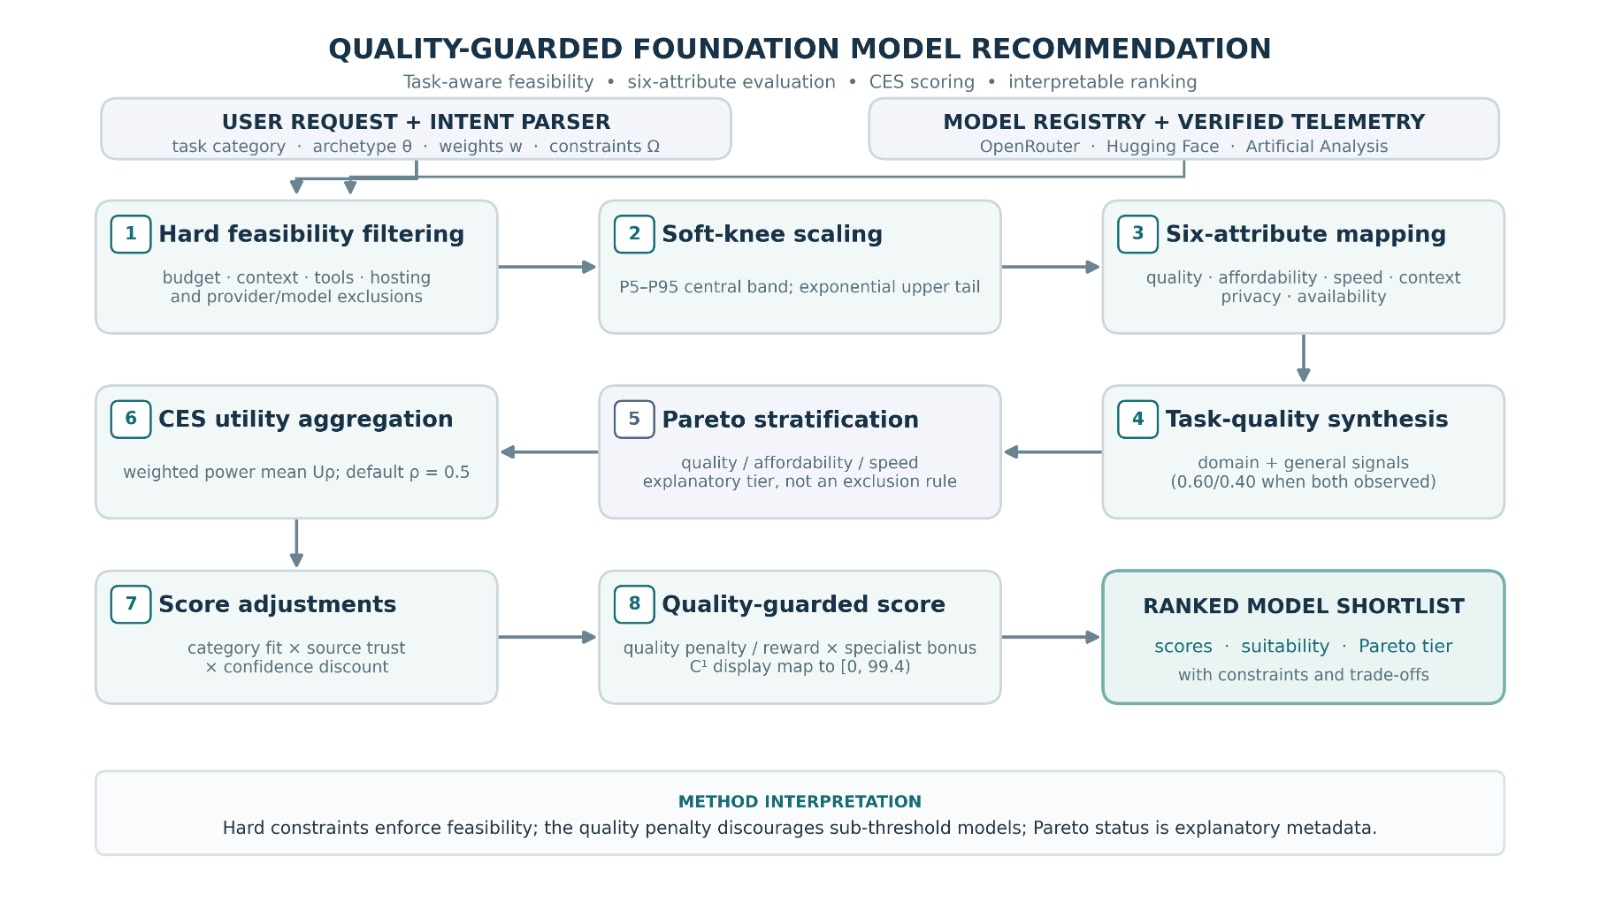
\includegraphics[width=\textwidth]{diagram.png}
\caption{Architecture of the proposed quality-guarded multi-attribute foundation model recommendation pipeline. Natural-language intent parsing identifies task priorities and operational constraints, while an integrated model registry supplies candidate attributes. Hard feasibility filtering, soft-knee normalization, and task-quality synthesis precede Pareto stratification over quality, affordability, and inference speed. The six-dimensional CES utility is combined with multiplicative scoring adjustments, archetype-dependent quality factors, and an asymptotic display ceiling to produce ranked recommendations. Pareto membership is retained as explanatory metadata and does not directly determine score order.}\label{fig:pipeline}
\end{figure}

Figure~\ref{fig:pipeline} illustrates the architecture of the proposed quality-guarded multi-attribute foundation model recommendation pipeline. The process begins with a natural-language user request, which is interpreted to identify the target task category, operational constraints, and attribute priorities. The intent-parsing component determines the corresponding operational archetype---frontier, balanced, budget, or speed---and generates a weight vector for six evaluation dimensions: task quality, affordability, inference speed, context capacity, privacy, and availability.

Candidate models are retrieved from the integrated model registry, which incorporates metadata and benchmark observations from OpenRouter, Hugging Face, and Artificial Analysis. Hard feasibility constraints are applied to exclude candidates that violate explicitly specified requirements. The remaining models are evaluated using normalized telemetry attributes, where soft-knee percentile normalization reduces sensitivity to outliers while preserving discrimination among high-performing models. Task-specific quality is synthesized from available domain-specific and general capability measurements.

Pareto stratification identifies non-dominated models using the quality--affordability--speed efficiency triplet. Importantly, Pareto membership serves as explanatory metadata rather than as a mandatory ranking or elimination criterion. Subsequently, the six normalized attributes are aggregated through a weighted constant-elasticity-of-substitution (CES) utility function, with the default parameter set to $\rho = 0.5$. The resulting utility is adjusted using category fit, source trust, confidence discounting, and task-specific specialization factors.

A continuous quality-deficit penalty discourages models with insufficient task proficiency, while the frontier archetype additionally incorporates a quality-dependent reward. Finally, a continuously differentiable asymptotic ceiling maps the adjusted score to a bounded scale below 99.4 without introducing upper-end ranking ties. The pipeline produces an ordered list of feasible models accompanied by their evaluation scores, attribute information, and Pareto membership, thereby supporting transparent, task-aware model selection.

The recommendation methodology operates as an eight-stage pipeline:
\begin{enumerate}
  \item Hard Operational Constraint Filtering ($\mathcal{M} \to \mathcal{M}^*$).
  \item Outlier-Robust Soft-Knee Percentile Cohort Normalization.
  \item Dimensional Telemetry Mapping.
  \item Dual-Signal Task Quality Synthesis.
  \item Multi-Objective Pareto Frontier Stratification.
  \item Concave CES Power-Mean Utility Aggregation ($U_\rho$).
  \item Cobb--Douglas Multiplicative Coupling and Confidence Discounting.
  \item Continuous Deficit Penalties, Frontier Rewards, and $C^1$ Asymptotic Display Ceiling.
\end{enumerate}

\subsection{Hard Operational Constraint Filtering}\label{subsec:filtering}

Prior to scalar scoring, candidates must satisfy the non-compensatory constraint set $\Omega$. The admissible space $\mathcal{M}^*$ is defined as:
\begin{equation}\label{eq:filtering}
\mathcal{M}^* = \{ m \in \mathcal{M} \mid \forall c_j \in \Omega : \phi(m, c_j) = 1 \},
\end{equation}
where the indicator predicate $\phi(m, c_j)$ enforces satisfaction across:
\begin{itemize}
  \item \textbf{Context Capacity:} $\text{ctx}_m \ge \text{ctx}_{\min}$.
  \item \textbf{Budget Ceiling:} If a price ceiling is specified it is applied to the input price alone, $P_m^{\text{in}} \le P_{\max}^{\text{in}}$, because the ceiling is stated per million input tokens and the input price is the term present for every priced model. A model whose input price is unlisted is retained: the predicate removes only models \emph{known} to breach the ceiling, absence of a price not being evidence of a high one. Two consequences are carried into the evaluation below: a workload dominated by output tokens can admit a model whose blended cost exceeds the stated ceiling, and an unpriced model is never removed by this predicate.
  \item \textbf{Governance and Self-Hosting:} Mandates for on-premises or air-gapped deployment strictly admit only open-source or open-weight models ($\text{access}_m \in \{\text{Open source}, \text{open-weights}\}$).
  \item \textbf{Modality and Tool Support:} Requires verified parameter support for function calling or structured outputs ($\mathcal{T}_{\text{req}} \subseteq \mathcal{T}_m$).
  \item \textbf{Provider/Model Exclusions:} $\text{provider}_m \notin \mathcal{P}_{\text{exclude}} \land \text{id}_m \notin \mathcal{M}_{\text{exclude}}$.
\end{itemize}
Constraint filtering represents the only absolute non-compensatory mechanism in the system.

\subsection{Outlier-Robust Soft-Knee Percentile Normalization}\label{subsec:normalization}

Let $v_{m, k}$ denote the raw observed telemetry value of model $m$ for metric dimension $k$ (e.g., benchmark indices from the \href{https://artificialanalysis.ai/api-reference}{Artificial Analysis API}, tokens per second, or context lengths). Standard min-max scaling is vulnerable to single-sample extremes, and hard-clipping at a fixed upper percentile $P_{95}$ collapses all top-tier models onto an identical $1.0$ score, causing \emph{tie-saturation} among precisely the candidates a procurement decision must discriminate. We therefore scale the central cohort linearly against its own percentile band and attach a soft exponential tail above the upper knee, giving the \emph{soft-knee percentile normalization} $\mathcal{N}(v; P_5, P_{95})$:
\begin{equation}\label{eq:normalization}
\mathcal{N}(v) = \begin{cases}
\kappa \left( \dfrac{v - P_5}{r} \right), & P_5 \le v \le P_{95}, \\[8pt]
\kappa + (1 - \kappa) \left( 1 - \exp\left( -\dfrac{v - P_{95}}{\tau_{\mathrm{tail}} r} \right) \right), & v > P_{95},
\end{cases}
\end{equation}
with $\mathcal{N}(v) = 0$ for $v < P_5$, where $r = P_{95} - P_5$ is the empirical 90\% inter-percentile range, $\kappa = 0.92$ sets the knee at $P_{95}$, and $\tau_{\mathrm{tail}} = 0.30$ is the tail scaling parameter (summarized in Table~\ref{tab:norm_params}).

\begin{table}[!htbp]
\caption{Parameters for soft-knee cohort normalization.}\label{tab:norm_params}
\centering
\small
\begin{tabularx}{\linewidth}{@{}p{2.4cm}X@{}}
\toprule
\textbf{Parameter} & \textbf{Operational Value and Design Rationale} \\
\midrule
$\kappa$ (Knee) & $0.92$ --- Value at $P_{95}$; reserves $8\%$ headroom for elite frontier differentiation. \\
$\tau_{\mathrm{tail}}$ (Tail Scale) & $0.30$ --- Tail reaches $1 - e^{-1} \approx 63.2\%$ of the remaining headroom at distance $\tau_{\mathrm{tail}} r$ above $P_{95}$. \\
$P_5$ (Saturation Point) & 5th cohort percentile; $\mathcal{N}$ saturates at $0$ below it, since the lower tail is dominated by failed or near-zero evaluations. \\
$P_{95}$ (Knee Point) & 95th cohort percentile; the linear limb spans $[P_5, P_{95}]$. \\
\bottomrule
\end{tabularx}
\end{table}

This formulation possesses four key mathematical properties:
\begin{enumerate}
  \item \textbf{Outlier Resistance:} The central 90\% of the distribution is scaled linearly against cohort percentiles rather than single-sample extremes.
  \item \textbf{Strict Rank-Order Monotonicity on $[P_5, \infty)$:} The normalization function $N(v)$ is continuous and strictly increasing
for $v \geq P_5$. Its derivative is strictly positive on the open intervals
$(P_5,P_{95})$ and $(P_{95},\infty)$, but the function is not differentiable
at the breakpoints $P_5$ and $P_{95}$. Consequently, for any
$v_1 > v_2 \geq P_5$, we have $N(v_1) > N(v_2)$.
In particular, the exponential upper-tail mapping assigns distinct
normalized values to models above $P_{95}$, thereby avoiding tie
saturation introduced by hard percentile clipping.
Below $P_5$, normalization saturates at zero by design.
Candidates in this region may receive a quality-deficit penalty
during scoring, as described in Section~\ref{subsec:deficits},
but are not automatically excluded unless they violate an
explicit hard feasibility constraint.
  \item \textbf{Cohort Invariance under Filter Shifts:} Percentiles $P_5, P_{95}$ are computed once over the entire ingested catalog rather than post-filter candidate subsets, guaranteeing that a candidate's normalized capability does not change merely because another model was filtered.
  \item \textbf{Continuity with slope changes at the saturation point and knee:} $\mathcal{N}$ is continuous but not differentiable at $P_5$, where the constant zero limb meets the positive-slope central limb, and at $P_{95}$, where its slope jumps from $\kappa / r$ on the linear limb to $(1 - \kappa)/(\tau_{\mathrm{tail}} r) = 0.267 / r$ on the exponential tail, an attenuation of roughly $71\%$. It is therefore $C^0$ but not $C^1$ at either join. The upper-knee slope change is deliberate---a softer tail would flatten the elite band the knee exists to separate---and is disclosed here because Section~\ref{sec:introduction} criticises step penalties. The frontier quality factor is continuously differentiable (\(C^1\)), whereas the balanced, budget, and speed quality factors are continuous (\(C^0\)) but not differentiable at their quality threshold. The asymptotic display ceiling is \(C^1\), and the coding-generalist quality adjustment is also \(C^1\) with respect to quality following the smoothstep revision described in Section~\ref{subsec:deficits}.
\end{enumerate}

\subsection{Dimensional Telemetry Formulations}\label{subsec:dimensions}

For each model $m \in \mathcal{M}^*$, the system evaluates six standardized coordinates $\mathbf{x}_m = [x_{m, \text{qual}}, x_{m, \text{aff}}, x_{m, \text{spd}}, x_{m, \text{ctx}}, x_{m, \text{priv}}, x_{m, \text{avail}}]^T \in [0, 1]^6$:

\subsubsection{Affordability ($x_{m, \text{aff}}$)}
Pricing is evaluated using a category-sensitive blended token cost. General work is weighted toward output tokens, whereas document and retrieval workloads are input-heavy:
\begin{equation}\label{eq:price_blend}
P_m^{\text{blend}} = \begin{cases}
0.60 P_m^{\text{in}} + 0.40 P_m^{\text{out}}, & \text{general work}, \\[4pt]
0.85 P_m^{\text{in}} + 0.15 P_m^{\text{out}}, & \text{document work}.
\end{cases}
\end{equation}
Because token costs span several orders of magnitude (from zero for open-source models to over \$50/M tokens for reasoning APIs), affordability is mapped logarithmically:
\begin{equation}\label{eq:price_map}
x_{m, \text{aff}} = \operatorname{clamp}\left( 1.0 - \frac{\log_{10}(P_m^{\text{blend}} + 1.0)}{2.1}, \; 0.45, \; 0.98 \right).
\end{equation}
For a positive blended price, the map is clamped to $[0.45,0.98]$; the upper bound is approached at the free-price end, and the lower bound binds from roughly \$13/M tokens upward. A non-positive or unavailable blended price is treated as unmeasured rather than as a measured free service. Newly imported open-weight models with unknown self-hosting infrastructure costs receive the explicit heuristic $x_{m,\text{aff}}=0.95$; for other records, a registry rebuild retains any previously stored affordability value, and a value still missing when scoring occurs receives the scorer's general missing-metric floor of $0.08$. These are distinct fallback paths: $0.95$ is an optimistic unknown-infrastructure-cost assumption, whereas $0.08$ is a conservative generic missing-value floor. In the frozen 47-model cohort, all 47 have positive blended prices and use the price map; zero use the $0.95$ open-weight fallback, and zero rely on a retained or missing-value fallback. Therefore, none of these unmeasured-price paths affects the budget panel.

\subsubsection{Context Capacity ($x_{m, \text{ctx}}$)}
Context capacity spans from $1\text{K}$ to $10\text{M}+$ tokens. The map is a linear-fractional (rational) function of $\log_{10}(\text{ctx})$ rather than a logistic one; its purpose is to compress the range while reserving resolution for the long-window regime:
\begin{equation}\label{eq:context_map}
x_{m, \text{ctx}} = \operatorname{clamp}\left( 1.55 \, \frac{\log_{10}(\text{ctx}_m) - 2.0}{\log_{10}(\text{ctx}_m) + 1.0}, \; 0.08, \; 1.0 \right),
\end{equation}
yielding $x_{\text{ctx}} \approx 0.54$ at $4\text{K}$, $0.71$ at $32\text{K}$, $0.79$ at $128\text{K}$, and $0.89$ at $1\text{M}$ tokens.

\subsubsection{Inference Speed ($x_{m, \text{spd}}$)}
Empirical output throughput $\text{Th}_m$ (tokens per second) from the \href{https://artificialanalysis.ai/api-reference}{Artificial Analysis API} is calibrated via:
\begin{equation}\label{eq:speed_map}
x_{m, \text{spd}} = \operatorname{clamp}\left( 0.25 + \frac{\text{Th}_m}{300} \cdot 0.73, \; 0.25, \; 0.98 \right),
\end{equation}
yielding $\approx 0.35$ at $40\text{ t/s}$, $\approx 0.54$ at $120\text{ t/s}$, and $0.98$ at $\ge 300\text{ t/s}$.

\subsubsection{Privacy and Availability ($x_{m, \text{priv}}, x_{m, \text{avail}}$)}
Privacy is a three-level classification of the access model, $x_{m,\text{priv}} \in \{1.0,0.75,0.45\}$ for self-hostable open weights, zero-data-retention hosted endpoints, and standard cloud APIs, respectively. Availability is a provider-level aggregate of catalogue presence, endpoint redundancy and SLA history, with every catalogue-listed provider scored $0.90$ in the revision this paper evaluates. Neither coordinate varies across the evaluation cohort ($\text{priv} = 0.45$, $\text{avail} = 0.90$ for all 47 models), so neither can move a ranking in any panel reported here, and both are recorded as classification rather than measurement for that reason; Section~\ref{subsec:weights} reports the span that makes this auditable.

\subsection{Dual-Signal Task Quality Synthesis}\label{subsec:quality}

In specialized workloads such as coding or agentic execution, relying solely on domain syntax pass rates yields incomplete evaluations. Real-world engineering requires both domain mastery and broad algorithmic reasoning.

Let $c_{\text{norm}}$ denote normalized domain execution capability (e.g., HumanEval, SWE-bench) and $i_{\text{norm}}$ denote normalized general cognitive intelligence (MMLU, Chatbot Arena Elo). The combined capability index is:
\begin{equation}\label{eq:dual_signal}
\tilde{c}_m = \begin{cases}
0.60 \, c_{\text{norm}} + 0.40 \, i_{\text{norm}}, & \text{if } c_{\text{norm}} \neq \emptyset \land i_{\text{norm}} \neq \emptyset, \\
c_{\text{norm}}, & \text{if } i_{\text{norm}} = \emptyset, \\
i_{\text{norm}}, & \text{if } c_{\text{norm}} = \emptyset.
\end{cases}
\end{equation}
The composite capability is then mapped into task quality via a concave curve:
\begin{equation}\label{eq:quality_curve}
x_{m, \text{qual}} = \operatorname{clamp}\left( 0.34 + 0.65 \sqrt{\tilde{c}_m}, \; 0.40, \; d \right), \quad d = \begin{cases} 0.99, & \text{coding capability}, \\ 0.98, & \text{overall quality}. \end{cases}
\end{equation}
The square-root transformation amplifies capability gains at lower thresholds while requiring substantial advances across both reasoning and code execution to approach the upper bound.

\subsection{Multi-Objective Pareto Frontier Stratification}\label{subsec:pareto}

Prior to scalar utility aggregation, candidates are evaluated for multi-objective Pareto optimality over their core efficiency triplet $\mathbf{y}_m = [x_{m, \text{qual}}, x_{m, \text{aff}}, x_{m, \text{spd}}]^T$:

\begin{definition}[Pareto Dominance]\label{def:pareto}
Model $m_a$ dominates model $m_b$ ($m_a \succ_{\mathcal{P}} m_b$) if and only if:
\begin{equation}\label{eq:pareto_def}
\forall j \in \{\text{qual}, \text{aff}, \text{spd}\}, \; y_{m_a, j} \ge y_{m_b, j} \quad \land \quad \exists k \in \{\text{qual}, \text{aff}, \text{spd}\}, \; y_{m_a, k} > y_{m_b, k}.
\end{equation}
\end{definition}

The candidate set is partitioned into two disjoint subsets:
\begin{align}
\mathcal{P}_{\text{frontier}} &= \{ m \in \mathcal{M}^* \mid \nexists m' \in \mathcal{M}^* : m' \succ_{\mathcal{P}} m \}, \label{eq:p_front} \\
\mathcal{P}_{\text{eligible}} &= \mathcal{M}^* \setminus \mathcal{P}_{\text{frontier}}. \label{eq:p_elig}
\end{align}
The partition is computed with the standard maxima-of-a-set procedure \cite{kung1975maxima}. Models in $\mathcal{P}_{\text{frontier}}$ are non-dominated alternatives that cannot be improved in quality, affordability, or speed without sacrificing another dimension. This Pareto tier is surfaced as explanatory metadata, so a user can audit which candidates are non-dominated in the efficiency triplet. It is \emph{not} a guarantee that frontier membership determines rank, and the difference is not cosmetic wherever a coordinate outside the triplet carries weight.

\subsubsection{The Pareto tier and the score rank in different spaces: a scope condition on the dominance proposition}\label{subsec:pareto_scope}

Definition~\ref{def:pareto} is stated over the triplet $\mathbf{y} = [x_{\text{qual}}, x_{\text{aff}}, x_{\text{spd}}]$, whereas the score $S(m)$ of Section~\ref{sec:theory} aggregates all six coordinates. Proposition~\ref{prop:dominance} bridges the two only under the hypothesis that every coordinate with positive weight lies in the triplet. The shipped frontier and budget profiles both violate that hypothesis by assigning context weight $0.20$ and $0.65$, respectively; the balanced profile also assigns context weight $0.65$. Outside the proposition's stated restriction, a model dominated on the triplet can still be preferred because of a positively weighted coordinate outside it.

A concrete case, using the square-root power mean of Eq.~\ref{eq:rho_half} with normalised weights $0.60$ on quality, $0.20$ on affordability and $0.20$ on context. Let $m_a$ have $(x_{\text{qual}}, x_{\text{aff}}, x_{\text{spd}}, x_{\text{ctx}}) = (0.90, 0.50, 0.50, 0.30)$ and $m_b$ have $(0.85, 0.45, 0.45, 0.90)$, with all other coordinates equal. Since each of the three triplet coordinates is strictly larger for $m_a$ and no coordinate is smaller, $m_a \succ_{\mathcal{P}} m_b$ by Definition~\ref{def:pareto}. The utilities are $U(m_a) = (0.60\sqrt{0.90} + 0.20\sqrt{0.50} + 0.20\sqrt{0.30})^2 = 0.673$ and $U(m_b) = (0.60\sqrt{0.85} + 0.20\sqrt{0.45} + 0.20\sqrt{0.90})^2 = 0.769$, so $m_b$ outranks $m_a$ despite being triplet-dominated. This does not contradict Proposition~\ref{prop:monotonicity}, which requires coordinate-wise dominance over the coordinates that carry weight and therefore does not apply when one model is better on context and worse on quality. It does mean that the two properties are separate ones: the concatenation of the Pareto filter with the score is not itself a dominance-consistent order, and citing frontier membership as a justification for a rank would be wrong. Frontier status is consequently reported throughout as metadata.

\subsection{Cobb--Douglas/CES Utility Aggregation}\label{subsec:ces}

Given normalized weights $\bar{w}_k = w_k / \sum_j w_j$ and attribute coordinates $x_{m, k} \in [0, 1]$, the multi-attribute utility is evaluated using the CES family:
\begin{align}
U_\rho(\mathbf{x}_m) &= \left( \sum_{k=1}^K \bar{w}_k x_{m, k}^\rho \right)^{1/\rho}, \quad 0 < \rho \le 1, \label{eq:ces_formula} \\
U_0(\mathbf{x}_m) &= \prod_{k=1}^K \max(x_{m, k}, \varepsilon)^{\bar{w}_k}, \quad \varepsilon = 0.05. \label{eq:cd_formula}
\end{align}
Our default configuration employs $\rho = 0.5$, which simplifies to the square-root power mean:
\begin{equation}\label{eq:rho_half}
U_{0.5}(\mathbf{x}_m) = \left( \sum_{k=1}^K \bar{w}_k \sqrt{x_{m, k}} \right)^2.
\end{equation}
By the generalized power-mean inequality \cite{hardy1934inequalities},
for $0 < \rho \leq 1$, the regularized Cobb--Douglas utility,
the CES utility, and the weighted arithmetic mean satisfy the
following ordering whenever $x_{m,k} \geq \varepsilon$ for every
attribute with positive weight $\bar{w}_k > 0$:

\begin{equation}\label{eq:jensen}
U_0(\mathbf{x}_m) \leq U_{\rho}(\mathbf{x}_m)
\leq U_1(\mathbf{x}_m)
= \sum_{k=1}^{K} \bar{w}_k x_{m,k}.
\end{equation}

Under this condition, the regularization floor in $U_0$ is inactive,
so the standard power-mean inequality applies. For $0 < \rho < 1$,
equality throughout holds if and only if all positively weighted
attribute values are equal. The operational attribute mappings in
Section~4.3 satisfy this condition because their minimum mapped
value is $0.08$, exceeding $\varepsilon = 0.05$. For counterfactual
values below $\varepsilon$, the inequality between the floored
Cobb--Douglas endpoint and the unfloored CES utility is not
guaranteed.

For the default choice $\rho = 0.5$, the elasticity of substitution
is $\sigma = 1/(1-\rho) = 2.0$. The resulting CES aggregator permits
more substitution than the Cobb--Douglas limit ($\sigma = 1$), but
penalizes attribute imbalances relative to the weighted arithmetic
mean. Unlike the unfloored Cobb--Douglas product, it remains
well-defined when an attribute is zero.
\subsection{Multiplicative Coupling and Confidence Discounting}\label{subsec:coupling}

Base utility is scaled into an initial raw score via multiplicative Cobb--Douglas coupling:
\begin{equation}\label{eq:base_score}
S_m^{\text{base}} = 100 \cdot U_m \cdot F_m^\alpha \cdot \gamma(C_m) \cdot T_m,
\end{equation}
where:
\begin{itemize}
  \item \textbf{Category Fit ($F_m$):} Measures alignment with the query category $\mathcal{C}^*$. A primary-use-case match gives $F_m = 1.00$ and a secondary match gives $0.88$; failing both, the category pairs give $1.00$ for an exact category match, $0.72$ for a general model applied to document work, $0.58$ for a document or voice model applied to general work, and $0.16$ for any other mismatch. With elasticity parameter $\alpha = 1.2$, an incompatible model is attenuated by $0.16^{1.2} \approx 0.11$.
  \item \textbf{Source Trust ($T_m$):} A multiplicative provenance factor, $T_m = \operatorname{clamp}(a_m \cdot r_m \cdot l_m, 0.45, 1.0)$, where $a_m$ is source authority ($1.00$ first-party, $0.99$ benchmark, $0.98$ aggregator or curated, $0.95$ seed, $0.85$ heuristic), $r_m$ is record type ($1.00$ API model, $0.98$ open-weight model, $0.95$ repository or model-family record) and $l_m$ is link health ($1.00$ verified, $0.98$ catalogue, $0.97$ unverified, $0.50$ broken). An unclassified record defaults to $0.98$ on each factor, and a hidden or non-deployable record type is scored $T_m = 0$ and removed from contention. The clamp floors the factor at $0.45$, so provenance can move a score by at most a factor of $2.2$.
  \item \textbf{Confidence Discount ($\gamma(C_m)$):} Metadata verification maturity $C_m \in [0, 1]$ is discounted quadratically:
  \begin{equation}\label{eq:confidence}
  \gamma(C_m) = 1.0 - \lambda (1.0 - C_m)^2, \quad \lambda = 0.20.
  \end{equation}
  This ensures $\gamma'(1.0) = 0$ (no variance penalty for fully verified models), while discounting unverified models by up to 20\% ($\gamma(0) = 0.80$).
\end{itemize}

\subsection{Continuous Quality Deficit Penalties and Frontier Rewards}\label{subsec:deficits}

To reduce compensation for a quality shortfall without introducing step-function cliff discontinuities, the frontier archetype uses a continuous rational deficit penalty:
\begin{equation}\label{eq:deficit_penalty}
\psi_{\text{frontier}}(q) = \frac{1}{1.0 + \lambda_f (q_f - q)_+^p},
\end{equation}
where $(q_f, \lambda_f, p) = (0.92, 3.0, 1.2)$. Balanced, budget, and speed use the shared logarithmic deficit factor $1/[1 + 1.8\ln(1 + 3.5(0.70-q)_+)]$, which is gentler for mild shortfalls.

For frontier queries, models meeting or exceeding the threshold ($q \ge 0.92$) receive a convex super-frontier ceiling reward:
\begin{equation}\label{eq:frontier_reward}
\beta(q) = 1.0 + 0.25 \left( \frac{q - 0.92}{0.08} \right)^{1.5}.
\end{equation}
Define the effective quality factor for all four archetypes $\theta\in\{\text{frontier},\text{balanced},\text{budget},\text{speed}\}$. For frontier, $g_{\text{frontier}}(q)=\psi_{\text{frontier}}(q)$ when $q<0.92$ and $g_{\text{frontier}}(q)=\beta(q)$ when $q\ge0.92$. For balanced, budget, and speed, $g_\theta(q)=1/[1+1.8\ln(1+3.5(0.70-q)_+)]$ for every $q$, which equals $1$ above the shared threshold. For frontier, $p=1.2>1$ makes the left derivative zero at the threshold, and the right derivative of $\beta$ is also zero, so $g_{\text{frontier}}$ is $C^1$. For the other three archetypes, the logarithmic limb meets the constant $1$ continuously with finite one-sided slope, so $g_\theta$ is $C^0$ and strictly increasing in quality below $0.70$. The implemented factor is therefore defined for all four values of $\theta$.

For coding queries in the general category, three specialisation terms stack additively: a coding-specialist weight ($+4\%$), chain-of-thought reasoning ($+3\%$) and agentic tool use ($+2\%$), so $B_m \le 1.09$. A generalist that is neither a code specialist nor a reasoning model receives a smooth quality factor. Define $t(q)=\operatorname{clip}((q-0.95)/0.05,0,1)$ and $h(t)=3t^2-2t^3$; then $B_m=0.92+0.08h(t(q))$. This factor is $0.92$ for $q\leq0.95$, reaches $1$ at $q=1$, and has zero derivative at both endpoints. The adjusted score is $S_m^{\text{adj}} = S_m^{\text{base}} \cdot g_\theta(x_{m, \text{qual}}) \cdot B_m$.

\textbf{Continuity of the coding quality factor.} The cubic smoothstep removes the former 8\% jump at $q=0.95$: the generalist coding factor is continuously differentiable with respect to quality at both $q=0.95$ and $q=1$. This statement concerns the quality-dependent factor; specialist and reasoning bonuses remain discrete metadata terms. All empirical tables were regenerated with this revised factor.

\subsection{Continuously Differentiable ($C^1$) Asymptotic Display Ceiling}\label{subsec:ceiling}

When high-quality models accumulate specialist bonuses and frontier rewards, composite scores can exceed 100. Applying a hard clip $\min(99, S)$ causes catastrophic score saturation, collapsing multiple elite models onto identical integer scores. We implement a smooth asymptotic exponential soft-ceiling:
\begin{equation}\label{eq:soft_ceiling}
\mathcal{C}(S) = \begin{cases}
S, & S \le s_0, \\[4pt]
s_0 + H \left( 1 - \exp\left( -\dfrac{S - s_0}{M} \right) \right), & S > s_0,
\end{cases}
\end{equation}
with knee threshold $s_0 = 86.0$, asymptotic headroom $H = 99.4 - 86.0 = 13.4$, and smoothing scale $M = 13.4$. Setting $M = H$ guarantees that the derivative is exactly 1.0 on both sides of the knee:
\begin{equation}\label{eq:c1_ceiling}
\lim_{S \to 86^-} \mathcal{C}'(S) = 1.0, \quad \lim_{S \to 86^+} \mathcal{C}'(S) = \frac{H}{M} e^0 = 1.0.
\end{equation}
Final recommendation scores lie strictly within $[0, 99.4)$, preserving the natural linear calibration below $86.0$ while guaranteeing strict rank monotonicity across the elite frontier.

\section{Theoretical Properties}\label{sec:theory}

Throughout this section, the full recommendation score is:
\begin{equation}
S(m) = \mathcal{C}\Big( 100 \cdot U_\rho(\mathbf{x}_m) \cdot F_m^\alpha \cdot \gamma(C_m) \cdot T_m \cdot g_\theta(x_{m, \text{qual}}) \cdot B_m \Big).
\end{equation}

\begin{proposition}[Monotonicity, Ceteris Paribus]\label{prop:monotonicity}
Let models $m_a, m_b$ share identical category fit $F$, confidence $C$, trust $T$, specialist bonus $B$, and archetype $\theta$. If $\mathbf{x}_{m_a} \ge \mathbf{x}_{m_b}$ coordinate-wise with $x_{m_a, k} > x_{m_b, k}$ for some attribute with priority weight $w_k > 0$, then $S(m_a) > S(m_b)$.
\end{proposition}

\begin{proof}
For $\rho \in (0, 1]$, the mapping $t \mapsto t^\rho$ is strictly increasing on $\mathbb{R}_+$. Let $k$ be the coordinate named in the hypothesis, so that $w_k > 0$ and hence $\bar{w}_k = w_k / \sum_j w_j > 0$, with $x_{m_a, k} > x_{m_b, k} \ge 0$. Then $\bar{w}_k x_{m_a, k}^\rho > \bar{w}_k x_{m_b, k}^\rho$, while for every $j \ne k$ the term is weakly larger, $\bar{w}_j x_{m_a, j}^\rho \ge \bar{w}_j x_{m_b, j}^\rho$, because $x_{m_a, j} \ge x_{m_b, j}$ and weights are non-negative. Summing, $\sum_j \bar{w}_j x_{m_a, j}^\rho > \sum_j \bar{w}_j x_{m_b, j}^\rho$, and raising to the strictly increasing power $1/\rho$ preserves the strict inequality. The argument uses only the existence of \emph{one} positively weighted coordinate that is strictly larger; coordinates with $w_j = 0$ contribute nothing to either side and the parsed vectors, which set some weights to zero, therefore satisfy the hypothesis. For $\rho = 0$ the same step applies to the floored product provided $x_{m_b, k} \ge \varepsilon$; every clamp in Section~\ref{subsec:dimensions} returns at least $0.08$, so this holds for every coordinate the pipeline maps. It does not hold for a coordinate set to zero by hand, which the pipeline never emits: the stress test of Section~\ref{subsec:ablation} does exactly that, and is labelled there as a counterfactual bound rather than as a state the method produces. The common factor $100 F^\alpha \gamma(C) T B > 0$ preserves ordering. Furthermore, since $x_{m_a, \text{qual}} \ge x_{m_b, \text{qual}}$ and $g_\theta(q) > 0$ is nondecreasing, $U g_\theta$ is strictly larger for $m_a$. Because the display ceiling $\mathcal{C}(S)$ has a strictly positive first derivative $\mathcal{C}'(S) > 0$ everywhere, $S(m_a) > S(m_b)$.
\end{proof}

\begin{proposition}[Dominance Consistency]\label{prop:dominance}
If all attributes with positive weights $w_k > 0$ belong to the efficiency triplet $\mathbf{y} = [x_{\text{qual}}, x_{\text{aff}}, x_{\text{spd}}]^T$ and $m_a \succ_{\mathcal{P}} m_b$ with equal $F, C, T, B$, then $S(m_a) \ge S(m_b)$. The inequality is strict when at least one strictly improved triplet coordinate has positive weight. Equality is possible when all positively weighted coordinates tie and the only strict gains are on zero-weight coordinates that do not change the quality factor (for example, an affordability-only gain when quality is unchanged).
\end{proposition}

\begin{proof}
By Definition~\ref{def:pareto}, $m_a \succ_{\mathcal{P}} m_b$ implies $\mathbf{y}_{m_a} \ge \mathbf{y}_{m_b}$ coordinate-wise. All positively weighted coordinates lie in this triplet, so the score cannot decrease, by the weak form of coordinate-wise monotonicity. If at least one strict gain is on a positively weighted coordinate, Proposition~\ref{prop:monotonicity} gives a strict score increase. If all positively weighted coordinates tie, equality follows when the quality factor also ties; a strict gain on a zero-weight quality coordinate can still increase the score through $g_\theta$, so it is not an equality case.
\end{proof}

\begin{proposition}[Quality-Conditional Score Ceiling]\label{prop:ceiling}
Suppose $F_m, \gamma(C_m), T_m, B_m \le 1.0$ and task quality $x_{m, \text{qual}} = q$. Then, regardless of the values of the other coordinates, the recommendation score is bounded by:
\begin{equation}\label{eq:ceiling_proof}
S(m) \le 100 g_\theta(q).
\end{equation}
\end{proposition}

\begin{proof}
Because $x_{m, k} \le 1.0$ for all $k$, $U_\rho(\mathbf{x}_m) \le 1.0$. Multiplicative factors satisfy $F^\alpha \gamma T B \le 1.0$. Furthermore, $\mathcal{C}(s) \le s$ since $H(1 - e^{-z/H}) \le z$. Thus, $S(m) \le S^{\text{base}} g_\theta(q) \le 100 g_\theta(q)$, completing the proof.
\end{proof}

For a frontier query with $q_f = 0.92, \lambda_f = 3.0, p = 1.2$, a model with quality $q = 0.89$ is capped at $95.7$, and a model with $q = 0.71$ is capped at $68.4$, even if its other coordinates are perfect ($1.0$). These examples instantiate the frontier penalty; $g_\theta$ gives the corresponding bound for balanced, budget, and speed. The proposition assumes $B_m\le1$ and therefore does not cover the coding-specialist bonus case ($B_m$ can reach $1.09$); the display ceiling still bounds the final score below $99.4$. Proposition~\ref{prop:monotonicity} separately establishes ordering under a common $B$.

\begin{proposition}[Non-Compensation of the Aggregator]\label{prop:agg_noncomp}
Let attribute $k$ have normalized weight $\bar{w}_k$ and $x_k = 0$. For $\rho \in (0, 1)$, $U_\rho \le (1 - \bar{w}_k)^{1/\rho}$. For $\rho = 0$ with floor $\varepsilon$, $U_0 \le \varepsilon^{\bar{w}_k}$; without the floor, $U_0 = 0$.
\end{proposition}

\begin{proof}
For $\rho \in (0, 1)$, $U_\rho = (\sum_{j \neq k} \bar{w}_j x_j^\rho)^{1/\rho} \le (\sum_{j \neq k} \bar{w}_j)^{1/\rho} = (1 - \bar{w}_k)^{1/\rho}$ since $x_j \le 1.0$. For $\rho = 0$, the $k$-th factor is $\varepsilon^{\bar{w}_k}$ and remaining factors are $\le 1.0$.
\end{proof}

\begin{proposition}[Properties of the Asymptotic Display Ceiling]\label{prop:ceiling_props}
The soft-ceiling $\mathcal{C}(S)$ is $C^1$ continuous on $\mathbb{R}$, strictly increasing, satisfies $\mathcal{C}(S) \le S$, and satisfies $\mathcal{C}(S) < 99.4$ for all finite $S$.
\end{proposition}

\begin{proof}
For $S \le s_0$, $\mathcal{C}'(S) = 1.0$. For $S > s_0$, $\mathcal{C}'(S) = \frac{H}{M} e^{-(S - s_0)/M} = e^{-(S - s_0)/H} \in (0, 1)$ since $M = H$. As $S \downarrow s_0$, $\mathcal{C}'(S) \to 1.0$. Hence the first derivative is continuous everywhere. The upper bound follows from $\lim_{S \to \infty} \mathcal{C}(S) = s_0 + H = 86.0 + 13.4 = 99.4$.
\end{proof}

\section{Empirical Evaluation and Validation}\label{sec:evaluation}

The empirical results measure outcome alignment with Agent Arena's cost-blind headline net-improvement proxy, not user satisfaction. The frontier-intent panel is the primary result because this proxy most closely matches a quality-first objective. Budget and balanced Arena-regret panels are boundary results: the proxy does not measure the cost-sensitive trade-offs those intents express. We therefore also report a secondary evaluation using one explicit cost-sensitive utility and the same hard cost constraints for every method.

\subsection{Evaluation Setup and Live Telemetry Sources}\label{subsec:eval_setup}

To ensure empirical validity, candidate alternatives are derived from our live registry store, which is populated with catalog metadata and token pricing from the \href{https://openrouter.ai/docs/api-reference/overview}{OpenRouter API}~\cite{openrouter2024} and with repository telemetry (architecture, licence, download and like counts) from the \href{https://huggingface.co/docs/hub/api}{Hugging Face API}~\cite{hf2023}. The repository telemetry informs model identity and the source-trust factor of Section~\ref{subsec:coupling} only; no evaluation outcome reported in this section is computed from it. Capability and throughput metrics are calibrated against benchmark observations from the \href{https://artificialanalysis.ai/api-reference}{Artificial Analysis API}~\cite{aa2024}, including Artificial Analysis Intelligence Indices, Coding Benchmark pass rates, and verified output throughput (tokens per second).

\subsection{Illustrative frontier-coding recommendation}\label{subsec:coding_case}

In the illustrative nine-model coding case, the parsed frontier profile assigns zero weight to affordability and ranks Claude Opus 5.5 first (score $98.32$); two sub-frontier controls are demoted by the continuous quality-deficit penalty. This example illustrates pipeline behavior only and is not evidence of user-preference satisfaction; the comparative evidence is the frozen-cohort evaluation below. The archive contains the analysis scripts but omits the frozen inputs and generated complete rankings described in the Data Availability statement.

\subsection{Exponent, missing-telemetry, and display stress tests}\label{subsec:ablation}

Across the nine-model exponent ablation, the ordering is unchanged for $\rho\in\{0,0.25,0.5,1\}$ ($r_s=1.00$). In a deliberately adversarial missing-context counterfactual, the $\rho=0.5$ score is $75.5$, compared with $69.2$ for regularized Cobb--Douglas; this is a stress test, not an operating missing-data state. The soft display ceiling preserves distinct scores for three high-scoring models ($98.32$, $97.49$, and $90.74$). Inverting the ceiling in Eq.~\ref{eq:soft_ceiling} gives pre-ceiling values of approximately $119.7$, $112.1$, and $91.9$, respectively; a hard cap at $99$ would collapse only the first two, while the third would remain at $91.9$. These tests characterize score behavior and do not establish comparative recommendation quality; the analysis scripts are in the research archive, while generated outputs and frozen inputs are omitted as described in the Data Availability statement.

\subsection{Outcome definition and provenance}\label{subsec:outcome}

The reference is the Agent Arena Overall leaderboard's headline net-improvement column. The payload also reports per-signal contrasts; an earlier extractor read the first signal rather than the headline. We corrected that provenance error, retained the original snapshot locally, and recomputed all reported panels from the headline column~\cite{arenaagent2026}. A separate harness defect ranked the proposed method on its \emph{rounded} display score while baselines used unrounded scores; all current analyses rank on the exact shipped score (\texttt{scoreExact}). Both corrections affect reported results and are disclosed; the analysis scripts and parser outputs are in the research archive, while the frozen payloads are withheld as described in the Data Availability statement.

The leaderboard's headline outcome $y_m$ is the equal-weighted mean of the per-model, per-signal treatment effects reported in the frozen payload; it is expressed in net-improvement percentage points. The 47-model cohort is evaluated at six per-task cost caps, $B_b\in\{\$0.10,\$0.25,\$0.50,\$1,\$2,\$5\}$. At each cap, the common eligible set $\mathcal{M}_b$ contains cohort models whose observed median Agent Arena task cost is no greater than $B_b$. For method $r$, $\hat m_{r,b}$ is its highest-ranked eligible model, and $m_b^*=\arg\max_{m\in\mathcal{M}_b}y_m$ is the outcome oracle. Per-tier regret is the oracle outcome minus the selected outcome; the reported mean gives each of the six tiers equal weight:
\begin{equation}\label{eq:regret}
R_{r,b}=y_{m_b^*}-y_{\hat m_{r,b}}=\max_{m\in\mathcal{M}_b}y_m-y_{\hat m_{r,b}},\qquad \overline{R}_r=\frac{1}{6}\sum_{b=1}^{6}R_{r,b}.
\end{equation}
Thus, $R_{r,b}=y_{m_b^*}-y_{\hat m_{r,b}}$ measures how far the recommendation falls below the best eligible outcome in that tier. This is outcome alignment with the cost-blind proxy, not user satisfaction; budget caps define eligibility, but the regret itself does not reward lower cost within a tier.

\subsection{Coverage of the catalogue}\label{subsec:coverage}

The outcome panels above are bounded by the leaderboard they grade: Agent Arena lists only models that appear in agentic traffic, so the cohort is the full intersection available at the time of retrieval rather than a sample of the catalogue~\cite{arenaagent2026}. Every recommendation in Sections~\ref{subsec:agent_validation}--\ref{subsec:cost_priced} is therefore a comparison of aggregation rules on the measured stratum, and none of them can say anything about a model the leaderboard does not list. The coverage statistic reported here is the complement of that statement: it is computed on the whole catalogue, it needs no outcome reference, and it records a property of the registry rather than of any aggregation rule.

\textbf{A tier is unserved when its top eligible record is structural.} Partition the catalogue into budget tiers by the maximum per-task cost an admissibility filter admits. Within each tier, rank the eligible records by the method's own score and take the top one. The tier is \emph{unserved} if that top record carries a structurally estimated capability score while a measured record was eligible to be chosen---that is, if the recommendation is forced to a model whose quality index rests on a specification rather than on a benchmark, not because no measured model qualifies, but because the measured models are ranked below the estimate. The statistic counts tiers, not models, because a single stale estimate can displace a measured model in every tier in which it is eligible.

\textbf{Repair moves the unserved tiers to zero.} Before repair, duplicate records for the same underlying model---the same checkpoint surfaced under more than one provider or effort variant---inflate the eligible set and let a structural estimate displace measured records it should not have competed against; the same duplication also discards confidence when two records disagree and neither provenance is preferred. After de-duplication against the registry and the assignment of a provenance-derived confidence to each remaining record, the number of unserved tiers falls from $4/24$ to $0/24$: on the repaired catalogue no budget tier has a structural estimate at its top while a measured record was eligible. The same repair moves unmeasured records inside the method's top ten from $8/40$ to $1/40$. Both figures are properties of the registry as repaired, and neither is a claim that the structural estimate is accurate where it is used; they say only that the regression to the estimate is no longer forced by a duplicate or an unresolved provenance conflict.

\textbf{Why this section needs no outcome.} An outcome-based panel can grade an aggregation rule only on the models the outcome covers, so the outcome panels of this paper are silent on the 366 of 671 catalogue records (54.5\%) whose score rests on a structural estimate; that stratum is in the catalogue but outside every leaderboard used here. The coverage statistic is the only evidence available for it, and because it is computed without an outcome it can be reported even where the outcome cannot. Its favourable direction is a consequence of the registry repair rather than of any method, and it is reported as such: it restores the measured stratum to the tiers from which duplicates had pushed it, and it does not demonstrate that a remaining structural estimate would outperform a measured model if one were eligible.

\subsection{Does Preference Integration Destroy Capability Alignment? Validation against Agent Arena}\label{subsec:agent_validation}

We first hold the intent fixed at the frontier, quality-maximising profile of Section~\ref{subsec:coding_case} and grade every method on the headline outcome. Table~\ref{tab:agent_validation} reports the result.

\begin{table}[!htbp]
\caption{Validation on the 2026-10-08 headline net-improvement column ($n{=}47$ distinct registry models): mean and worst-tier recommendation regret over per-task budgets $\$0.10$--$\$5.00$, paired 95\% bootstrap percentile interval for $\Delta_{P-M}$, defined as proposed mean regret minus method mean regret (2{,}000 model resamples), Spearman $r_s$ with a 95\% bootstrap interval, Kendall $\tau_b$, and the fraction of the outcome's top three models contained in the method's top three. \textbf{Bold} marks the best \emph{integrative} rule in the mean-regret column; the quality-only row is a cost-blind reference ordering. An interval containing zero means the gap is unresolved by this cohort. The composite is scored on its full six-coordinate profile with category fit, confidence discount and trust, whereas every baseline is scored on the three-coordinate triplet; Section~\ref{subsec:parity} measures how much of the difference that asymmetry accounts for.}\label{tab:agent_validation}
\centering
\footnotesize
\setlength{\tabcolsep}{2pt}
\begin{tabular*}{\linewidth}{@{\extracolsep{\fill}}lcccccc@{}}
\toprule
\textbf{Decision Method} & \textbf{Mean Regret} & \textbf{Worst} & \textbf{$\Delta_{P-M}$ (95\% CI)} & \textbf{$r_s$ (95\% CI)} & \textbf{$\tau_b$} & \textbf{Top-3} \\
\midrule
Proposed ($\rho{=}0.5$)    & \textbf{0.09} & \textbf{0.27} & --- & 0.816 $[0.649,0.911]$ & 0.650 & 2/3 \\
WSM (Linear)               & 0.49 & 2.38 & $[-0.40,\;1.96]$ & \textbf{0.837} $[0.676,0.922]$ & 0.674 & 1/3 \\
WSM + Hard Floor           & 0.49 & 2.38 & $[-2.12,\;1.64]$ & 0.785 $[0.612,0.895]$ & 0.643 & 1/3 \\
TOPSIS                     & 0.49 & 2.38 & $[-0.40,\;1.96]$ & 0.836 $[0.680,0.922]$ & 0.673 & 1/3 \\
Cobb--Douglas ($\rho{=}0$) & 0.49 & 2.38 & $[-0.40,\;1.96]$ & 0.830 $[0.669,0.916]$ & 0.661 & 1/3 \\
CES only (no fit/penalty) & 0.49 & 2.38 & $[-0.40,\;1.96]$ & 0.835 $[0.675,0.921]$ & 0.671 & 1/3 \\
\midrule
Quality only (ref.)        & 0.09 & 0.27 & $[-0.22,\;2.03]$ & 0.838 $[0.680,0.926]$ & 0.680 & 1/3 \\
\bottomrule
\end{tabular*}
\end{table}

Three findings follow. In Table~\ref{tab:agent_validation}, $\Delta_{P-M}$ is proposed mean regret minus method mean regret; the displayed intervals are paired 95\% bootstrap percentile intervals over model resamples. Point estimates equal to a confidence-interval endpoint can occur in this discrete resampling distribution.
\begin{itemize}
  \item \textbf{Under a capability-first intent the composite leads the original unpenalized integrative rules on point-estimate regret, but ties the matched WSM variant.} It attains mean regret $0.09$ and worst-tier regret $0.27$, versus $0.49$ and $2.38$ for the strongest original baseline values; captures $0.989$ of the tier oracle versus $0.943$; and attains the oracle at four of six tiers versus three for each original baseline. WSM with both the deficit factor and frontier reward also has mean regret $0.09$, although its top-three overlap is $1/3$. A separate descriptive value-for-money check gives the composite and quality-only ordering the same $24.2$ net-improvement points per dollar, with neither recommendation dominated in any tier. Every paired regret interval contains zero, so these are unresolved point-estimate differences. Section~\ref{subsec:parity} shows that removing the deficit factor alone leaves mean regret unchanged; removing the frontier reward raises it to $1.28$.
  \item \textbf{Rank fidelity is undifferentiated, and the reference ordering is nominally the best predictor.} Spearman correlations lie in $[0.785,0.838]$ with heavily overlapping intervals; the linear sum is nominally highest at $0.837$, the proposed score is $0.816$, and every interval contains the others. The quality-only ordering reaches $0.838$ with mean regret $0.09$. This is the expected behaviour of a cost-blind outcome and not evidence about the aggregator: net improvement prices neither cost nor latency, so the regret-minimising ordering of an admissible set is the quality ordering up to proxy noise, and any rule that spends weight on affordability or speed forfeits fidelity here \emph{by construction}. The quality-only row is therefore reported as a reference ordering rather than entered in the comparison.
  \item \textbf{The composite's shortlist fidelity is its clearest descriptive advantage in this panel.} Its top three contains two of the outcome's three highest-ranked models ($2/3$), whereas each original baseline places one there ($1/3$). Spearman is not a lead: WSM is $0.837$ and the proposed score is $0.816$. The linear-aggregator ablation has the same mean regret ($0.09$) and the same shortlist overlap ($2/3$); therefore, this cohort does not show a regret or top-three overlap improvement attributable to the CES aggregator. Removing the deficit factor leaves regret unchanged, while removing the frontier reward raises it; the paired interval for the latter difference includes zero. WSM with the deficit factor and TOPSIS with the deficit factor both remain at $0.49$ mean regret. These are cohort-specific comparisons, not evidence of a general causal effect. The shortlist statistic is coarse and needs external replication.
\end{itemize}

\subsection{Component Ablation and Baseline Parity}\label{subsec:parity}

Two questions bound the capability-first panel, and this subsection answers both on the same frozen cohort.

\textbf{Are the baselines handicapped?} The composite is scored on six coordinates with category fit, a confidence discount and a source-trust factor; the initial baselines are scored on the three-coordinate efficiency triplet. Table~\ref{tab:component_ablation} therefore re-runs each baseline on the same six coordinates with the same parsed weights. The six-coordinate and triplet variants attain identical mean regret, worst-tier regret and value captured ($0.49$, $2.38$ and $0.943$); the frontier profile assigns $0.20$ to context, $0.05$ to privacy, and $0.15$ to availability outside the triplet, or $0.40/(3.60+0.05+0.20+0.05+0.15)=9.9\%$ of its nominal weight. These coordinates move no tier's pick in this panel. This parity check addresses coordinate coverage, but does not show that CES is responsible for the proposed score's lead.

\textbf{Which component changes the result?} Table~\ref{tab:component_ablation} separates the below-threshold deficit factor from the frontier reward. Removing the deficit factor while retaining the reward leaves mean regret at $0.09$ and changes no tier pick; removing the reward while retaining the deficit factor changes two of six picks and raises mean regret to $1.28$ (paired difference versus the full score $1.19$, 95\% interval $[0,2.49]$). Removing both also gives $1.28$. Thus the old ablation attributed the change to the wrong component: on this cohort the point-estimate difference tracks the frontier reward, not the deficit factor, and its paired interval includes zero. WSM plus the deficit factor and TOPSIS plus the deficit factor each retain all six baseline picks and remain at $0.49$. Adding both the deficit factor and frontier reward to WSM changes one pick and gives $0.09$, but its top-three overlap remains $1/3$; the corresponding TOPSIS variant remains at $0.49$. Under budget and balanced intents, adding the production deficit factor to WSM or TOPSIS changes no tier picks or mean regrets (WSM $6.66$ and $0.79$; TOPSIS $5.10$ and $1.52$, respectively). Replacing the power mean by a linear aggregator leaves mean regret unchanged at $0.09$ and retains top-three overlap at $2/3$, matching the full pipeline. The confidence discount, category fit and source trust each move mean regret by less than $0.005$ on this cohort. Under budget intent, removing the specialist bonus improves regret from $9.07$ to $6.66$, another cohort-specific result rather than a general mechanism.

\begin{table}[!htbp]
\caption{Corrected component ablation and matched-penalty baseline comparison on the frozen cohort ($n{=}47$, 2026-10-08 headline column), under the capability-first intent of Table~\ref{tab:agent_validation}. WSM and TOPSIS use the same six normalized benefit coordinates and pinned weights; the deficit factor is the production archetype-specific multiplicative quality factor below threshold. The combined frontier variant also applies the above-threshold reward. $\Delta$ is each row's mean regret minus the full-pipeline mean; its 95\% percentile interval uses 2{,}000 paired model bootstrap resamples with the tier oracle recomputed. Mean and worst are regret in net-improvement points; lower is better.}\label{tab:component_ablation}
\centering
\footnotesize
\setlength{\tabcolsep}{2pt}
\begin{tabular*}{\linewidth}{@{\extracolsep{\fill}}lcccccc@{}}
\toprule
\textbf{Variant} & \textbf{Mean} & \textbf{Worst} & \textbf{Value capt.} & \textbf{$\Delta$ (95\% CI)} & \textbf{$r_s$} & \textbf{Top-3} \\
\midrule
Full pipeline (shipped)            & \textbf{0.09} & \textbf{0.27} & \textbf{0.989} & --- & 0.816 & \textbf{2/3} \\
minus deficit (reward retained)    & 0.09 & 0.27 & 0.989 & $0.00\;[0.00,0.00]$ & 0.795 & 2/3 \\
minus frontier reward              & 1.28 & 4.77 & 0.851 & $1.19\;[0.00,2.49]$ & 0.763 & 2/3 \\
minus deficit and reward           & 1.28 & 4.77 & 0.851 & $1.19\;[0.00,2.49]$ & 0.731 & 2/3 \\
linear aggregator                  & 0.09 & 0.27 & 0.989 & $0.00\;[0.00,0.00]$ & 0.817 & 2/3 \\
\midrule
WSM (six coordinates)              & 0.49 & 2.38 & 0.943 & $0.40\;[-1.96,0.40]$ & 0.838 & 1/3 \\
WSM + deficit                      & 0.49 & 2.38 & 0.943 & $0.40\;[-1.96,0.40]$ & 0.835 & 1/3 \\
WSM + deficit + reward             & \textbf{0.09} & \textbf{0.27} & \textbf{0.989} & $0.00\;[-2.03,0.09]$ & 0.836 & 1/3 \\
TOPSIS (six coordinates)           & 0.49 & 2.38 & 0.943 & $0.40\;[-1.96,0.40]$ & 0.836 & 1/3 \\
TOPSIS + deficit                   & 0.49 & 2.38 & 0.943 & $0.40\;[-1.96,0.40]$ & 0.836 & 1/3 \\
TOPSIS + deficit + reward          & 0.49 & 2.38 & 0.943 & $0.40\;[-1.96,0.48]$ & 0.837 & 1/3 \\
\bottomrule
\end{tabular*}
\end{table}

\subsection{Intent-Conditioned Regret across Archetypes}\label{subsec:archetype_regret}

The purpose of the method is intent-conditioned recommendation, and the preceding test holds the intent fixed. We therefore repeat the analysis under three requests---\emph{``best frontier coding models''}, \emph{``budget coding models''} and \emph{``balanced coding models''}---all parsed by the hosted intent parser of Section~\ref{sec:problem}. The parser returns the target category and an ordered priority list; the archetype classifier maps the request onto one of four weight profiles, and the priority list determines the vector when no archetype is named. The requests resolve on the shipped implementation to frontier (quality $3.60$, affordability $0$, speed $0.05$, context $0.20$, privacy $0.05$, availability $0.15$), budget (affordability $2.50$, quality $0.85$, speed $0.60$, context $0.65$, privacy $0.05$, availability $0.05$), and balanced (quality $1.25$, affordability $0.05$, speed $0.05$, context $0.65$, privacy $0.05$, availability $0.05$) profiles. The proposed score uses the full parsed vector; triplet baselines use the quality, affordability, and speed projection, so these original panels compare bundled scoring and coordinate choices. The vectors and parser outputs are pinned in the research artifact. Section~\ref{subsec:parser_eval} summarizes parser reliability; the cohort and budget tiers are as in Section~\ref{subsec:agent_validation}.

\begin{table}[!htbp]
\caption{Mean regret, worst-tier regret and value captured under the \emph{budget} intent (prompt ``budget coding models''; parsed weights: affordability $2.50$, quality $0.85$, speed $0.60$, context $0.65$, privacy $0.05$, availability $0.05$) on the 2026-10-08 headline column. Regret is in net-improvement points; lower regret, higher value captured and a shorter worst tier are better. Each $\Delta$ interval is proposed regret minus method regret, using paired bootstrap resampling of models (95\% percentile interval). \textbf{Bold} marks the best integrative rule.}\label{tab:regret_budget}
\centering
\footnotesize
\setlength{\tabcolsep}{2pt}
\begin{tabular*}{\linewidth}{@{\extracolsep{\fill}}lcccccc@{}}
\toprule
\textbf{Decision Method} & \textbf{Mean Regret} & \textbf{Worst} & \textbf{Value captured} & \textbf{$\Delta_{P-M}$ (95\% CI)} & \textbf{$r_s$} & \textbf{$\tau_b$} \\
\midrule
Proposed ($\rho{=}0.5$)    & 9.07 & 15.30 & $-0.057$ & --- & $-0.602$ & $-0.430$ \\
WSM (Linear)               & \textbf{6.66} & 12.40 & 0.225 & $[-14.88,\;5.33]$ & $-0.582$ & $-0.404$ \\
WSM + Hard Floor           & 9.64 & 15.30 & $-0.123$ & $[-4.21,\;6.31]$ & 0.386 & 0.226 \\
TOPSIS                     & \textbf{5.10} & \textbf{10.54} & 0.406 & $[-11.45,\;5.26]$ & $-0.622$ & $-0.447$ \\
Cobb--Douglas ($\rho{=}0$) & \textbf{5.10} & \textbf{10.54} & 0.406 & $[-11.45,\;5.26]$ & $-0.623$ & $-0.441$ \\
CES only                   & \textbf{6.66} & 12.40 & 0.225 & $[-11.45,\;6.18]$ & $-0.584$ & $-0.410$ \\
\midrule
Quality only (ref.)        & 0.09 & 0.27 & 0.989 & $[3.22,\;14.31]$ & 0.838 & 0.680 \\
\bottomrule
\end{tabular*}
\end{table}

\begin{table}[!htbp]
\caption{Mean regret, worst-tier regret and value captured under the \emph{balanced} intent (prompt ``balanced coding models''; parsed weights: quality $1.25$, affordability $0.05$, speed $0.05$, context $0.65$, privacy $0.05$, availability $0.05$) on the 2026-10-08 headline column. Regret is in net-improvement points; lower regret, higher value captured and a shorter worst tier are better. Each $\Delta$ interval is proposed regret minus method regret, using paired bootstrap resampling of models (95\% percentile interval). \textbf{Bold} marks the best integrative rule on mean regret.}\label{tab:regret_balanced}
\centering
\footnotesize
\setlength{\tabcolsep}{2pt}
\begin{tabular*}{\linewidth}{@{\extracolsep{\fill}}lcccccc@{}}
\toprule
\textbf{Decision Method} & \textbf{Mean Regret} & \textbf{Worst} & \textbf{Value captured} & \textbf{$\Delta_{P-M}$ (95\% CI)} & \textbf{$r_s$} & \textbf{$\tau_b$} \\
\midrule
Proposed ($\rho{=}0.5$)    & 3.06 & 7.68 & 0.644 & --- & 0.604 & 0.430 \\
WSM (Linear)               & \textbf{0.79} & 2.38 & 0.908 & $[-0.40,\;7.70]$ & 0.760 & 0.573 \\
WSM + Hard Floor           & \textbf{0.79} & 2.38 & 0.908 & $[-1.01,\;7.70]$ & 0.701 & 0.534 \\
TOPSIS                     & 1.52 & 4.41 & 0.822 & $[-2.31,\;8.04]$ & 0.765 & 0.586 \\
Cobb--Douglas ($\rho{=}0$) & 6.47 & 16.43 & 0.246 & $[-5.75,\;4.61]$ & 0.693 & 0.523 \\
CES only                   & 1.73 & 5.90 & 0.799 & $[-0.40,\;6.76]$ & 0.736 & 0.558 \\
\midrule
Quality only (ref.)        & 0.09 & 0.27 & 0.989 & $[0.17,\;8.64]$ & 0.838 & 0.680 \\
\bottomrule
\end{tabular*}
\end{table}

These budget and balanced tables are boundary results for alignment with the cost-blind Arena outcome. On that outcome, the proposed method's regret is $9.07$ under budget (versus $5.10$ for TOPSIS and Cobb--Douglas) and $3.06$ under balanced (versus $0.79$ for WSM and floored WSM). The comparisons preserve the shipped parsed profiles and are not evidence about which method better satisfies cost-sensitive users. In the next analysis, all methods are instead graded with the same explicit cost-sensitive utility.

\subsection{Shared cost-sensitive utility evaluation}\label{subsec:shared_utility}

As a secondary outcome independent of the Arena net-improvement column, we evaluated every ranking on the same four normalized attributes: predicted coding quality $q_m$, log-inverse observed Agent Arena median session cost $c_m$, speed $s_m$, and context $x_m$. The common linear utility is
\begin{equation}\label{eq:shared_utility}
U_{m,p}=\sum_{k\in\{q,c,s,x\}}\tilde w_{p,k}z_{m,k},\qquad \sum_k\tilde w_{p,k}=1,
\end{equation}
where $z_{m,k}$ are min--max normalized over the frozen 47-model cohort (cost uses $1-\log(C_m/C_{\min})/\log(C_{\max}/C_{\min})$). The budget utility uses normalized weights $(0.1848,0.5435,0.1304,0.1413)$ for quality, cost utility, speed, and context, taken from the parsed budget profile. The parser supplied no explicit balanced weights for these four evaluation attributes, so balanced uses the equal-weight assumption $(0.25,0.25,0.25,0.25)$. Neither vector is validated against observed user choices. Every method first receives the same hard eligibility filter, observed median task cost $\leq B_b$, for each of the six caps $B_b$ defined above. Utility regret is $\max_{m\in\mathcal M_b}U_{m,p}-U_{\hat m_{r,b},p}$, averaged equally over the six tiers. We also report arithmetic mean quality, mean observed session cost, and the number of selected tier recommendations dominated on quality and cost (lower cost and at least equal quality, with one strict).

\begin{table}[!htbp]
\caption{Common cost-sensitive utility results on the frozen 47-model cohort. Every method uses the same hard observed-cost cap within each tier and is graded by the same intent-specific utility. Utility regret is averaged over six tiers; quality is the mean normalized quality; cost is mean observed median session cost in USD; dominated reports quality--cost Pareto-dominated selected tiers. The proposed row is the harmonized re-scoring of the proposed method using the shared observed-cost utility, rather than its shipped score. WSM's zero regret for both profiles follows by construction because it maximizes the same linear utility over each eligible set.}
\label{tab:shared_utility}
\centering
\footnotesize
\setlength{\tabcolsep}{4pt}
\begin{tabular*}{\linewidth}{@{\extracolsep{\fill}}llcccc@{}}
\toprule
\textbf{Intent} & \textbf{Method} & \textbf{Utility regret} & \textbf{Mean quality} & \textbf{Mean cost (USD)} & \textbf{Dominated tiers} \\
\midrule
Budget & Proposed (harmonized) & 0.0231 & 0.8481 & 0.0520 & 6/6 \\
       & WSM                   & 0.0000 & 0.9247 & 0.0738 & 0/6 \\
       & TOPSIS                & 0.0105 & 0.8983 & 0.0750 & 3/6 \\
       & Cobb--Douglas         & 0.0139 & 0.9205 & 0.1163 & 5/6 \\
       & CES ($\rho=0.5$)      & 0.0000 & 0.9247 & 0.0738 & 0/6 \\
\midrule
Balanced & Proposed (harmonized) & 0.0181 & 0.8969 & 0.2138 & 6/6 \\
         & WSM                   & 0.0000 & 0.9349 & 0.3517 & 5/6 \\
         & TOPSIS                & 0.0074 & 0.9097 & 0.2175 & 5/6 \\
         & Cobb--Douglas         & 0.0000 & 0.9349 & 0.3517 & 5/6 \\
         & CES ($\rho=0.5$)      & 0.0000 & 0.9349 & 0.3517 & 5/6 \\
\bottomrule
\end{tabular*}
\end{table}

The ``Proposed (harmonized)'' row retains the full scoring pipeline and intent-specific four-axis weights, replacing catalogue-price affordability with normalized observed session-cost utility. In this offline harness, both prompts use the balanced archetype; thus the proposed budget row also receives the shared balanced/budget/speed quality-deficit penalty, rather than a budget-specific archetype penalty. The dominated-tiers count compares only predicted quality and observed session cost, so it ignores speed and context. WSM is also dominated at 5/6 balanced tiers, so 6/6 versus 5/6 is not a meaningful gap.

The proposed harmonized ranking has nonzero shared-utility regret for both profiles and its selected recommendations are quality--cost dominated at all six tiers. Under balanced weights it has lower mean cost than the alternatives but also lower mean quality; the scalar utility expresses the chosen trade-off, while the dominance count exposes quality--cost inefficiency without assigning a weight. WSM's zero regret for each profile is an optimizer check rather than independent comparative evidence. These descriptive estimates share the cohort and observed cost source, have no user-preference ground truth or uncertainty interval, and should be treated as a secondary evaluation rather than independent external validation.

\subsection{Parser reliability and weight diagnostics}\label{subsec:parser_eval}

Across 17 prompts parsed four times, 16 returned identical categories, priority lists, and derived weights on all runs; one varied in a single run, changing its context/privacy priorities. Category was stable for all 17. Paraphrase tests exposed archetype-classification instability for budget and latency requests, so repeatability of the evaluated prompts does not establish invariance to wording or fidelity to user intent. The archive includes the pinned parser outputs used by the reported panels; full per-repeat and paraphrase diagnostics are not included.

\subsection{Nominal weights and realized influence}\label{subsec:weights}

Nominal weights do not directly equal realized influence after normalization, nonlinear transforms, and multiplicative factors. For this 47-model cohort, privacy and availability are constant and cannot affect any reported ranking. The archive includes a script to compute per-coordinate influence from the frozen inputs; because those inputs are withheld, the resulting decomposition is not included here.

\subsection{Cost and value-for-money results}\label{subsec:cost_priced}

The cost-sensitive Arena-regret panels are boundary results rather than evidence of intent satisfaction. Under the separate common-utility evaluation (Table~\ref{tab:shared_utility}), the harmonized proposed ranking has nonzero utility regret and is quality--cost dominated at all six selected tiers for both profiles. Under balanced weights it recommends lower-cost models on average, with lower mean quality than WSM, Cobb--Douglas, and CES. The utility analysis adds cost, quality, and Pareto evidence to the cost-blind outcome alignment, but remains descriptive because its weights are researcher-specified and its cost and quality inputs come from the same frozen cohort.

\FloatBarrier

\section{Discussion and Limitations}\label{sec:discussion}

The formal results establish properties of the scoring functions under their stated assumptions; they do not establish that the chosen profiles reflect user preferences. The primary empirical claim is narrow: on this cohort, the shipped method has the lowest capability-first point-estimate regret among integrative baselines, with paired intervals containing zero. Budget and balanced Arena-regret results are boundary comparisons against a proxy that omits cost-sensitive trade-offs. The common-utility analysis addresses that gap by applying the same explicit utility and hard cost caps to every method, but the proposed harmonized ranking has nonzero utility regret and is quality--cost dominated at all six tiers for each profile. The utility weights are assumptions rather than observed preferences, so neither analysis establishes intent satisfaction.

Several implementation and study limits matter. The parser is hosted and its outputs are recorded rather than regenerated. The evaluation uses one dated 47-model cohort and six nested budget tiers, so the effective number of independent decisions is small and uncertainty intervals are wide; we reuse one inspected cohort for all analyses, so this is not a temporal holdout. Privacy and availability are constant across the 47 models, so their ranking effects are untested. The Arena cohort does not cover the full catalogue; coverage describes registry behavior but cannot validate structurally estimated quality. Prices may be missing or stale, and the current budget filter uses input price rather than blended per-task cost. The matched ablation applies the same six-coordinate weights and production deficit factor to WSM and TOPSIS, and tests the frontier reward separately; it does not transfer category fit, confidence discount, source trust, or the coding-specialist adjustment to those baselines. Simple maximum-quality-under-a-common-budget and lexicographic rules are not evaluated. No independent expert or direct pairwise preference study is available. Telemetry maps and penalty constants are not comprehensively calibrated. The parser outputs and analysis scripts are in the accompanying archive; frozen third-party inputs are omitted as described in the Data Availability statement.

\subsection{Threats to validity}\label{subsec:threats}

The main threats are outcome-column dependence, snapshot dependence, small and nested tier counts, parser instability, incomplete catalogue coverage, untested privacy and availability variation, and the absence of user or expert preference ground truth. There is no temporal holdout or direct pairwise-choice cohort. The scripts document the extractor and rounded-ranking corrections; frozen payloads are not redistributed. Capability-first differences remain unresolved point estimates; no claim of human-preference validation is made. Further fully factor-matched comparisons, incorporating category fit, confidence discounting, source trust, and coding-specialist adjustments, together with simple cost-feasible decision rules, are needed before attributing improvements to the aggregation design.

\subsection{Scope of the claims}\label{subsec:claims}

Mean regret against Agent Arena's outcome is an outcome-alignment measure; because that outcome is cost-blind, it cannot establish intent fidelity for budget or balanced requests. We therefore add a common-utility evaluation with the same hard cost constraints for every method and report utility regret, cost, quality, and Pareto dominance. This is stronger evidence about cost-sensitive trade-offs than the Arena panels alone, but its researcher-specified weights and shared cohort limit the claim. Direct pairwise choices from budget and balanced users remain the appropriate next validation.

\section{Conclusion}\label{sec:conclusion}

This paper presents a foundation-model recommendation pipeline that combines hard feasibility constraints, Pareto stratification, CES aggregation, a continuous quality-deficit penalty, and a bounded display mapping. We prove monotonicity, a quality-conditional score ceiling, and display-ceiling properties under stated assumptions, and show by counterexample that Pareto-tier membership does not determine score rank when coordinates outside the efficiency triplet carry weight.

On a frozen 47-model Agent Arena cohort, the pipeline attains mean regret $0.09$ under capability-first intent, versus $0.49$ for the original unpenalized WSM and TOPSIS baselines; paired intervals include zero. WSM with both matched quality factors ties the pipeline at $0.09$. Corrected ablation shows that removing the deficit factor leaves mean regret at $0.09$ and changes no tier pick, whereas removing the frontier reward changes two of six picks and raises mean regret to $1.28$; the paired interval for this difference includes zero. Adding the deficit factor alone to WSM or TOPSIS leaves mean regret at $0.49$ and changes no baseline pick. The WSM variant with both factors has top-three overlap of $1/3$; the corresponding TOPSIS variant remains at $0.49$. Under budget and balanced intents, adding the deficit factor to either baseline changes no tier picks or mean regrets. Replacing the power mean with a linear aggregator leaves mean regret unchanged and retains top-three overlap at $2/3$, matching the full pipeline in this cohort. These results identify a cohort-specific point-estimate pattern, not a general causal advantage. Under budget and balanced intents the pipeline trails several baselines ($9.07$ versus $5.10$ under budget, and $3.06$ versus $0.79$ under balanced intent). Because the outcome prices neither cost nor latency, these comparisons identify a weakness against the available proxy and do not establish what a cost-sensitive user would prefer.

In the secondary shared-utility evaluation, the harmonized proposed scorer has mean utility regret of $0.0231$ for budget and $0.0181$ for balanced intent; its recommendations are quality--cost dominated in all six tiers for both profiles. These values use explicit evaluation weights, not observed user preferences.

The study is limited to one dated cohort and six budget tiers; telemetry maps and penalty constants are not comprehensively calibrated; privacy and availability are constant in the cohort; and parser outputs are recorded rather than regenerated. We therefore claim outcome alignment under capability-first intent, not user-intent satisfaction. Future work includes temporal validation, direct pairwise preference studies involving budget- and balanced-intent users, validation of shared-utility weights against observed user choices, and fully factor-matched baseline comparisons.

\bmhead{Funding}
This research received no specific grant from any funding agency in the public, commercial, or not-for-profit sectors.

\bmhead{Data availability}
The accompanying \texttt{Model-Compass-Research} source archive contains the analysis code and the recorded intent-parser outputs, but it does not contain the frozen model registry or the Agent Arena snapshots used for the reported tables. The two local Arena snapshots were produced by parsing the leaderboard's rendered-page payload; the current \href{https://help.arena.ai/articles/5629909088-terms-of-use?lang=en}{Arena Terms of Use} restrict automated extraction and redistribution of service output. We therefore do not redistribute those snapshots or claim that the archive alone reproduces the numerical results. Arena's publisher separately provides a historical leaderboard dataset through Hugging Face under CC BY 4.0 (\url{https://huggingface.co/datasets/lmarena-ai/leaderboard-dataset}); we have not established that its released records are equivalent to the specific frozen headline values used here, so it is not presented as a drop-in reproduction input. The registry also contains observations from OpenRouter, Hugging Face, and Artificial Analysis and is not bundled. The exact external repository/DOI is not deposited for this version. The hosted parser is not rerun: the frozen parser outputs are included in the archive.\href{https://doi.org/10.5281/zenodo.23507047}{Zenodo}

\bmhead{AI use in manuscript preparation}
AI assisted with manuscript formatting and language editing to improve readability, presentation, and clarity. .

\bmhead{Code availability}
The analysis code is supplied in the accompanying \texttt{Model-Compass-Research} source archive. It preserves the scoring implementation used for the reported analyses; the live application has since evolved, and its current registry and scores are not the basis of these paper results. No public repository URL or DOI has been deposited for this version. The archive includes the frozen analysis scripts and parser outputs but excludes the third-party snapshots and registry described above; running the full analyses therefore requires those exact inputs to be obtained through an authorized route. The archive's \texttt{LICENSE} file states the current reuse terms for the authors' code; third-party material remains subject to its own terms.\href{https://doi.org/10.5281/zenodo.23507047}{Zenodo}

\bmhead{Declarations}
The authors declare that they have no competing financial or non-financial interests that are directly or indirectly related to the work submitted for publication.

\clearpage
\FloatBarrier



\clearpage
\FloatBarrier

\begin{thebibliography}{99}

\bibitem{arrow1961capital}
Arrow, K.J., Chenery, H.B., Minhas, B.S., Solow, R.M.: Capital-labor substitution and economic efficiency. \emph{The Review of Economics and Statistics} \textbf{43}(3), 225--250 (1961). \href{https://doi.org/10.2307/1927286}{doi:10.2307/1927286}

\bibitem{aa2024}
Artificial Analysis: LLM quality, speed, and pricing benchmarks API (2024). \href{https://artificialanalysis.ai/api-reference}{https://artificialanalysis.ai/api-reference}. Accessed 30 September 2026

\bibitem{arenaagent2026}
Arena: Agent Arena leaderboard: net improvement and median cost per task. \href{https://arena.ai/leaderboard/agent}{https://arena.ai/leaderboard/agent} and \href{https://arena.ai/leaderboard/agent/pareto}{https://arena.ai/leaderboard/agent/pareto}. Payload last updated 8 October 2026, retrieved 11 October 2026

\bibitem{arena2025}
LMArena: Arena leaderboard dataset (\texttt{lmarena-ai/leaderboard-dataset}). Hugging Face (2026). \href{https://huggingface.co/datasets/lmarena-ai/leaderboard-dataset}{https://huggingface.co/datasets/lmarena-ai/leaderboard-dataset}

\bibitem{bommasani2021opportunities}
Bommasani, R., et al.: On the opportunities and risks of foundation models. arXiv preprint arXiv:2108.07258 (2021). \href{https://arxiv.org/abs/2108.07258}{arXiv:2108.07258}

\bibitem{brans1985preference}
Brans, J.P., Vincke, P.: A preference ranking organisation method: the PROMETHEE method for multiple criteria decision-making. \emph{Management Science} \textbf{31}(6), 647--656 (1985). \href{https://doi.org/10.1287/mnsc.31.6.647}{doi:10.1287/mnsc.31.6.647}

\bibitem{chen2021evaluating}
Chen, M., et al.: Evaluating large language models trained on code. arXiv preprint arXiv:2107.03374 (2021). \href{https://arxiv.org/abs/2107.03374}{arXiv:2107.03374}

\bibitem{chen2023frugalgpt}
Chen, L., Zaharia, M., Zou, J.: FrugalGPT: How to use large language models while reducing cost and improving performance. arXiv preprint arXiv:2305.05176 (2023). \href{https://arxiv.org/abs/2305.05176}{arXiv:2305.05176}

\bibitem{cobbe2021gsm8k}
Cobbe, K., et al.: Training verifiers to solve math word problems. arXiv preprint arXiv:2110.14168 (2021). \href{https://arxiv.org/abs/2110.14168}{arXiv:2110.14168}

\bibitem{cobb1928theory}
Cobb, C.W., Douglas, P.H.: A theory of production. \emph{The American Economic Review} \textbf{18}(1), 139--165 (1928). \href{https://doi.org/10.2307/1811556}{doi:10.2307/1811556}

\bibitem{hardy1934inequalities}
Hardy, G.H., Littlewood, J.E., P\'olya, G.: \emph{Inequalities}. Cambridge University Press, Cambridge (1934)

\bibitem{hendrycks2020measuring}
Hendrycks, D., et al.: Measuring massive multitask language understanding. In: \emph{International Conference on Learning Representations (ICLR)} (2021). \href{https://openreview.net/forum?id=d7KBjmI3GmQ}{openreview:d7KBjmI3GmQ}

\bibitem{hf2023}
Hugging Face: Open LLM Leaderboard and Hub API. Hugging Face Spaces (2024). \href{https://huggingface.co/docs/hub/api}{https://huggingface.co/docs/hub/api}

\bibitem{hwang1981multiple}
Hwang, C.L., Yoon, K.: \emph{Multiple Attribute Decision Making: Methods and Applications}. Springer, Berlin (1981). \href{https://doi.org/10.1007/978-3-642-48318-9}{doi:10.1007/978-3-642-48318-9}

\bibitem{jimenez2023swe}
Jimenez, C.E., et al.: SWE-bench: Can language models resolve real-world GitHub issues? In: \emph{International Conference on Learning Representations (ICLR)} (2024). \href{https://openreview.net/forum?id=shMODneKD4}{openreview:shMODneKD4}

\bibitem{kaplan2020scaling}
Kaplan, J., et al.: Scaling laws for neural language models. arXiv preprint arXiv:2001.08361 (2020). \href{https://arxiv.org/abs/2001.08361}{arXiv:2001.08361}

\bibitem{keeney1993decisions}
Keeney, R.L., Raiffa, H.: \emph{Decisions with Multiple Objectives: Preferences and Value Trade-Offs}. Cambridge University Press, Cambridge (1993). \href{https://doi.org/10.1017/CBO9780511983832}{doi:10.1017/CBO9780511983832}

\bibitem{kung1975maxima}
Kung, H.T., Luccio, F., Preparata, F.P.: On finding the maxima of a set of vectors. \emph{Journal of the ACM} \textbf{22}(4), 469--476 (1975). \href{https://doi.org/10.1145/321892.321899}{doi:10.1145/321892.321899}

\bibitem{ong2024routellm}
Ong, I., et al.: RouteLLM: Learning to route LLMs with preference data. arXiv preprint arXiv:2406.18665 (2024). \href{https://arxiv.org/abs/2406.18665}{arXiv:2406.18665}

\bibitem{openrouter2024}
OpenRouter: Unified API and model benchmarks endpoint (2024). \href{https://openrouter.ai/docs/api-reference/overview}{https://openrouter.ai/docs/api-reference/overview}. Accessed 30 September 2026

\bibitem{opricovic2004compromise}
Opricovic, S., Tzeng, G.-H.: Compromise solution by MCDM methods: A comparative analysis of VIKOR and TOPSIS. \emph{European Journal of Operational Research} \textbf{156}(2), 445--455 (2004). \href{https://doi.org/10.1016/S0377-2217(03)00020-1}{doi:10.1016/S0377-2217(03)00020-1}

\bibitem{roy1968classement}
Roy, B.: Classement et choix en pr\'esence de points de vue multiples (la m\'ethode ELECTRE). \emph{Revue Fran\c{c}aise d'Informatique et de Recherche Op\'erationnelle} \textbf{2}(8), 57--75 (1968). \href{https://doi.org/10.1051/ro/196802V100571}{doi:10.1051/ro/196802V100571}

\bibitem{saaty1980analytic}
Saaty, T.L.: \emph{The Analytic Hierarchy Process}. McGraw-Hill, New York (1980)

\bibitem{tversky1972elimination}
Tversky, A.: Elimination by aspects: A theory of choice. \emph{Psychological Review} \textbf{79}(4), 281--299 (1972). \href{https://doi.org/10.1037/h0032955}{doi:10.1037/h0032955}

\bibitem{zheng2024judging}
Zheng, L., et al.: Judging LLM-as-a-judge with MT-Bench and Chatbot Arena. In: \emph{Advances in Neural Information Processing Systems (NeurIPS)} (2023). \href{https://proceedings.neurips.cc/paper_files/paper/2023/hash/91f18a1287b30030061e38b76c8c4599-Abstract-Conference.html}{NeurIPS:2023}

\end{thebibliography}

\end{document}
